We now present results.  For the true flow, we take $L_{x}=10$
\[
\eta(x,0) = \cos(\tilde{x}), ~ q(x,0) = \sin(\tilde{x}), ~ \tilde{x} = \frac{\pi}{L_{x}}x,
\]
and use a pseudo-spectral scheme with $K_{T}=256$ modes and a 4th-order Runge--Kutta scheme with an integrating factor and time step $dt=10^{-2}$. We take $\epsilon=.1$ and $\mu=\sqrt{\epsilon}$.  The number of terms used in the DNO expansion is $M=14$, which generally ensures machine precision accuracy for relatively long time evolutions.  As for how we assimilate data, we set the variance $\sigma=.1$, and the number of ensemble members $N_{e}=3200$.  We truncate the DNO expansions at $M=1$ in part to allow for the effect of far lower order models to be seen in the data analysis process.  We take a sampling rate in time of $dt_{s}=.5$, which is 50 times that of the time step of the full numerical solver.  We likewise though use a 4th-order Runge--Kutta scheme with an integrating factor in order to perform the analysis to forecast update.  In order to provide comparisons, we then look at two simulations, one in which we have four equally spaced pressure plates in the domain $[-10,10]$, and one in which we have eight.  We then run the simulation to $t_{f}=20$, which given the choice of $\epsilon$, is a long enough period of time for nonlinear effects to create significant distortions of the original wave profile.  

The results of this are seen in the Figure \ref{fig:Mval_1}.  In Figure \ref{fig:Mval_1} (a) we compare the pointwise approximations generated by using four and eight pressure plate measurements compared to the true profile, $\eta_{tr}(x,t_{f})$.  In Figure \ref{fig:Mval_1} (b), we plot a histogram of $\log_{10}|\eta_{a}(x,t) - \eta_{tr}(x,t)|$, where $\eta_{a}(x,t)$ comes from either the four plate or eight plate measurements.  Finally, we look at the root-mean square error, 
\[
\left(\frac{\sum_{j=0}^{2K-1} \left( \eta_{tr}(x_{j},t) - \eta_{a}(x_{j},t) \right)^{2}}{\sum_{j=0}^{2K-1}\eta_{tr}^{2}(x_{j},t)}\right)^{1/2}, ~ x_{j} = -L_{x} + j\frac{L_{x}}{K},
\]
at each sampling time in Figure \ref{fig:Mval_1} (c).  As one would expect, we get markedly better estimates by using twice the number of pressure plate based height measurements.  
\begin{figure}
\centering
\begin{tabular}{c}
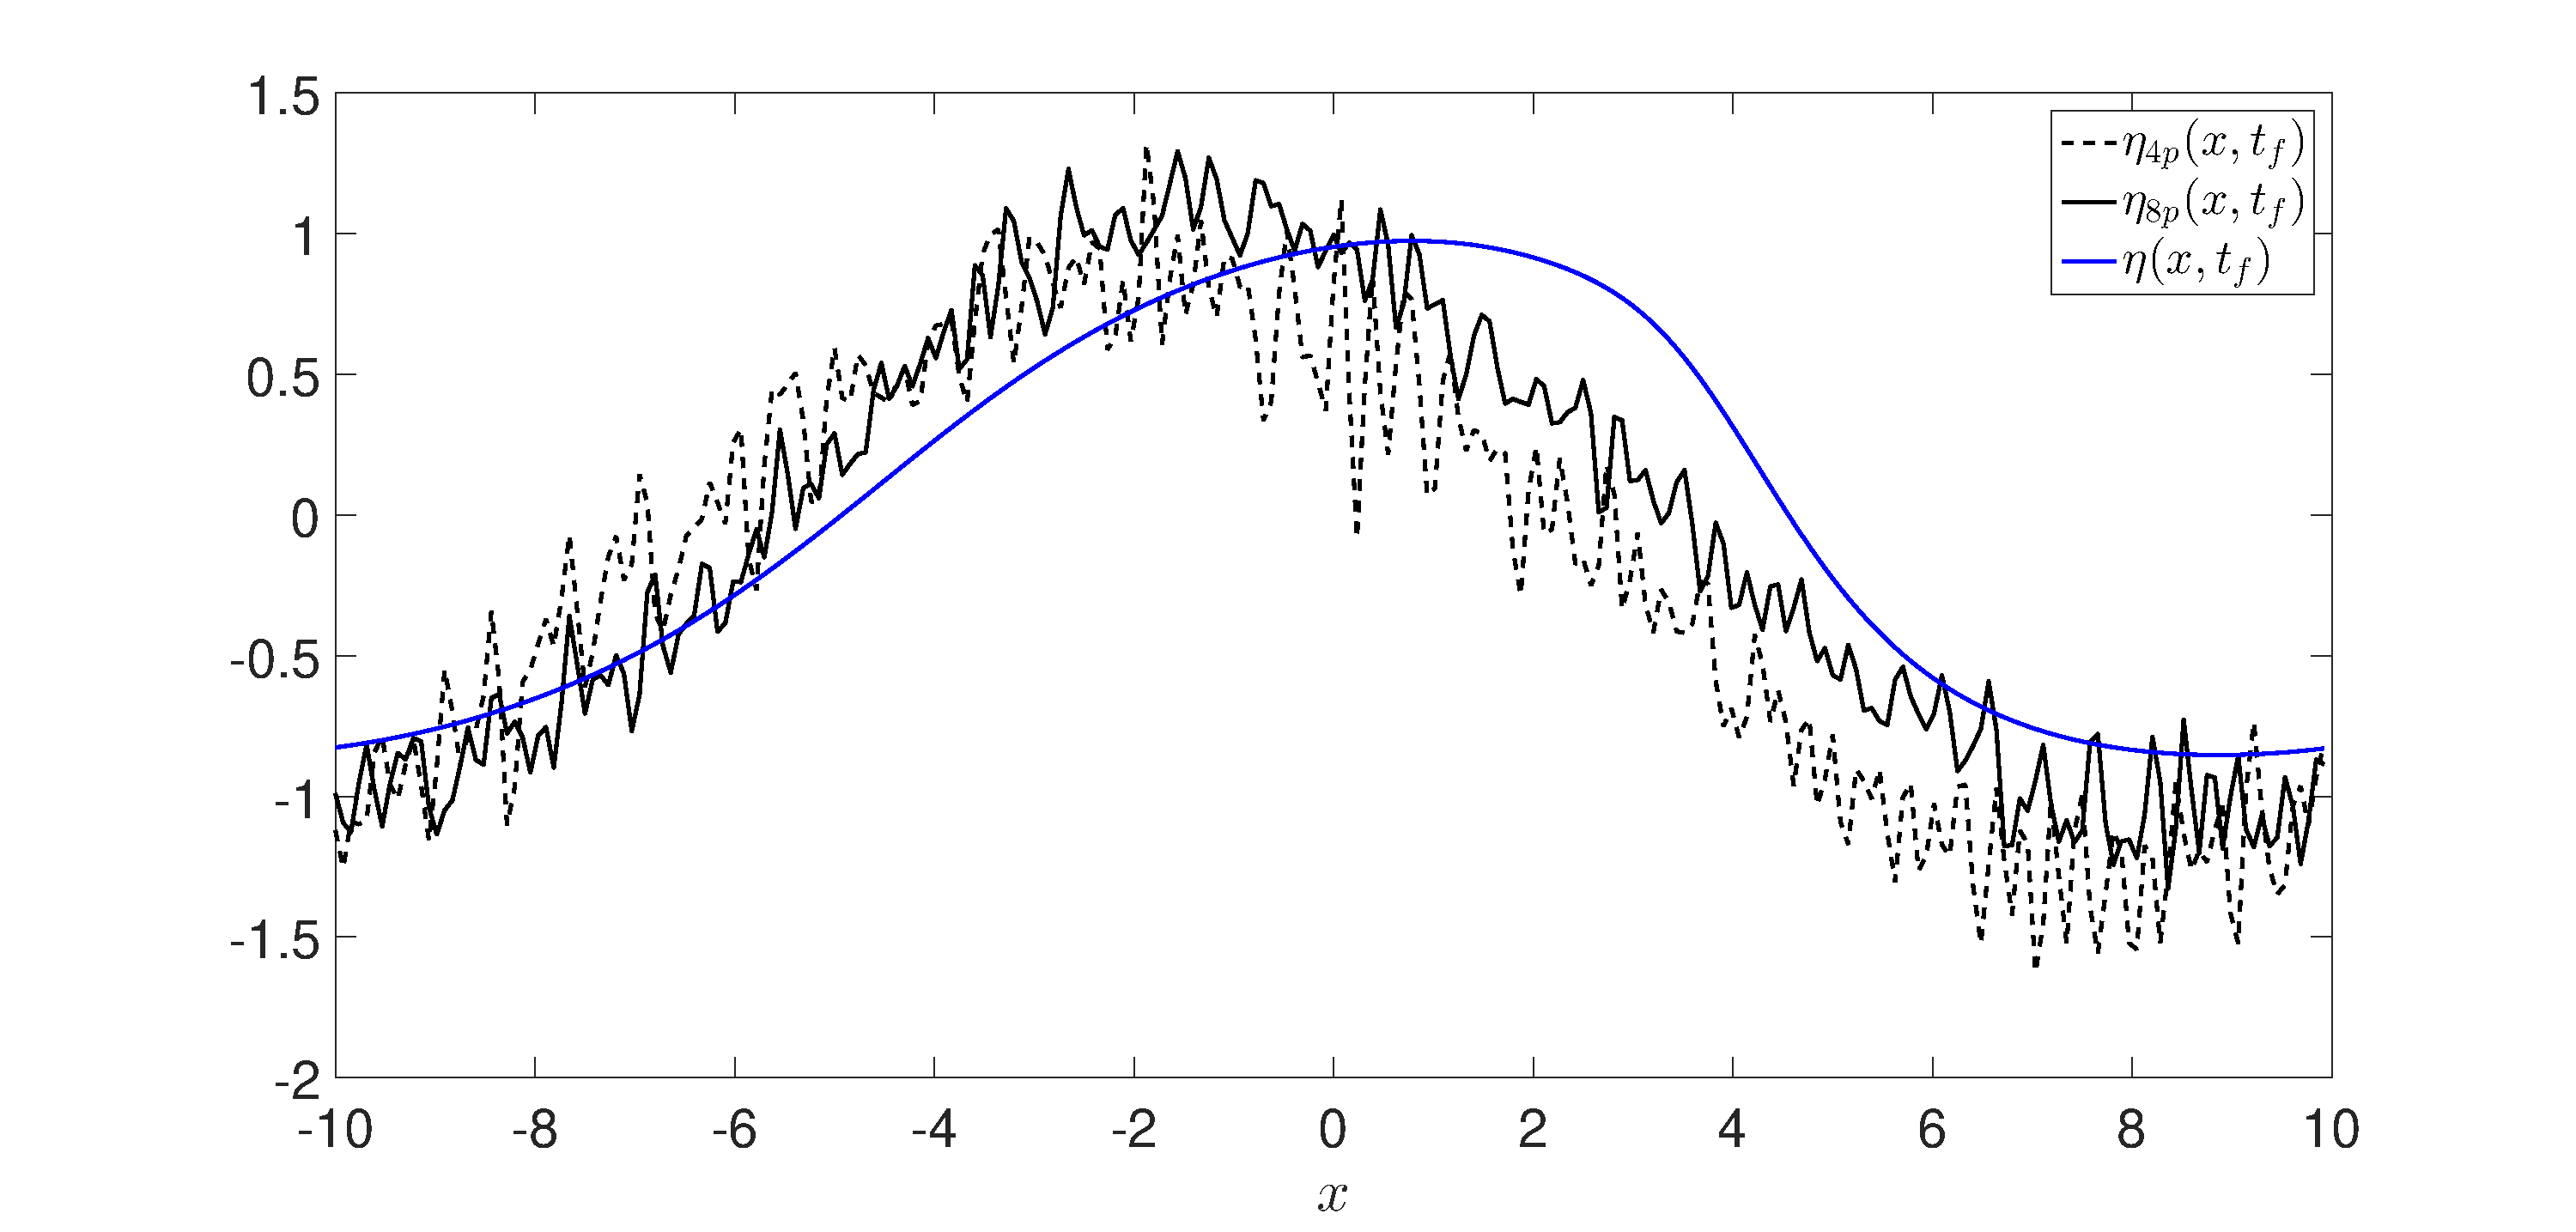
\includegraphics[width=.95\textwidth]{Images/wave_tf_20_sig_pt1_4_vs8pplates_Mval_1} \\
(a)\\
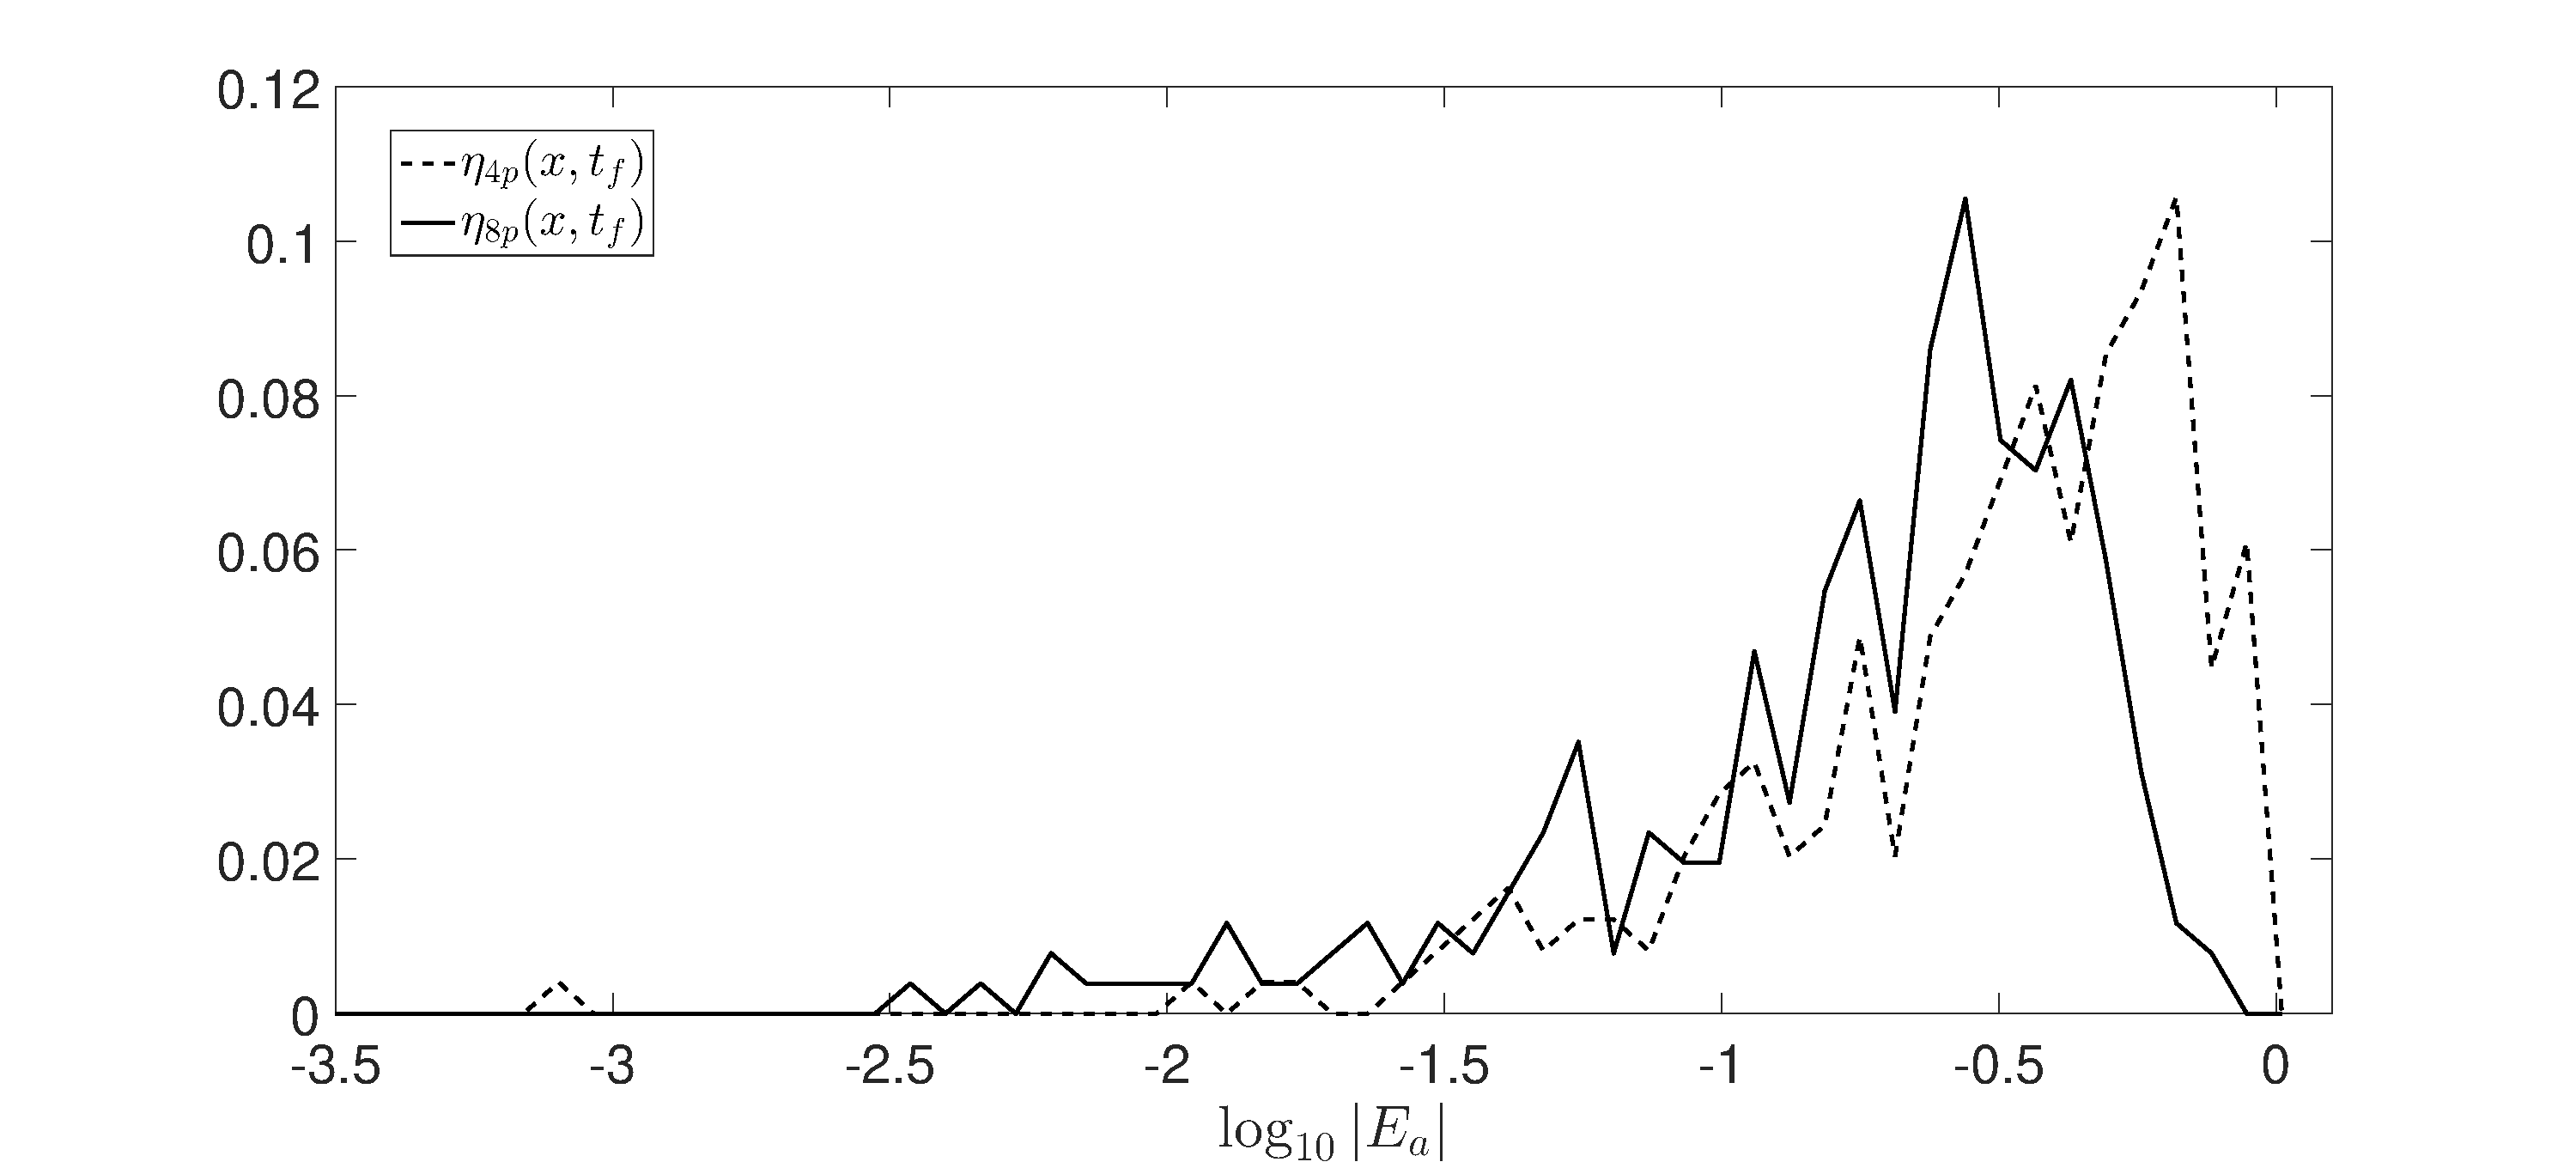
\includegraphics[width=.95\textwidth]{Images/histogram_tf_20_sig_pt1_4_vs8pplates_Mval_1}\\
(b)\\
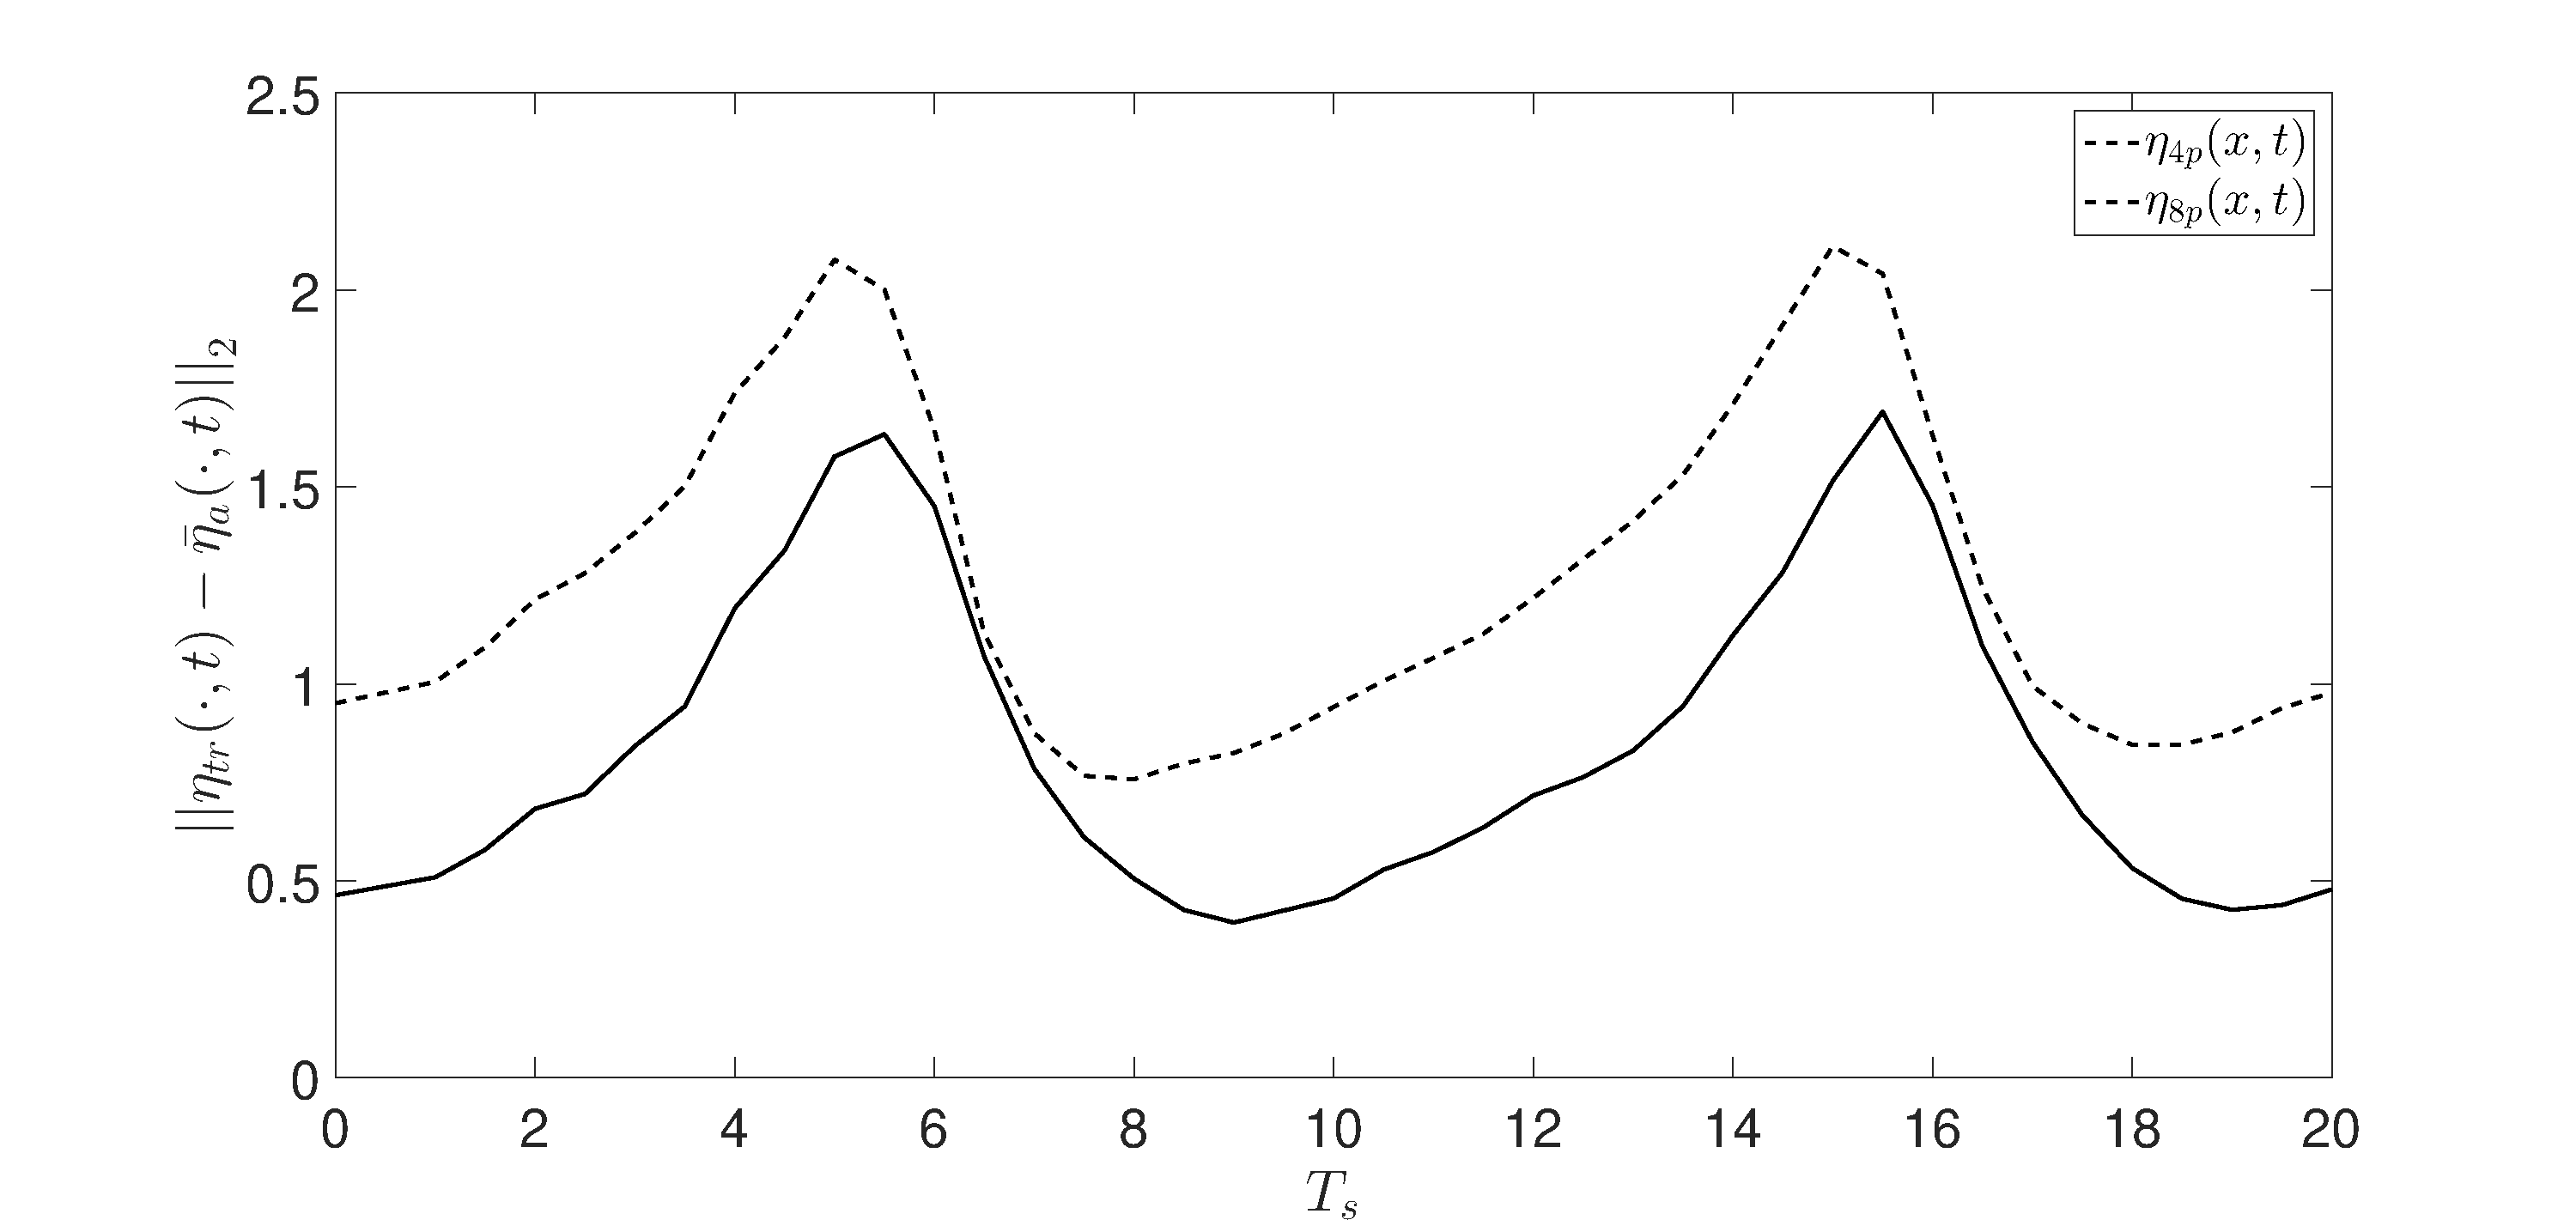
\includegraphics[width=.95\textwidth]{Images/rmserr_tf_20_sig_pt1_4_vs8pplates_Mval_1}\\
(c)
\end{tabular}
\caption{For $M=1$, $dt_{s}=.5$, with four plates (--) compared to eight (-), we have the wave profiles at $t_{f}=20$ (a), a histogram of the log of the pointwise error (b), and the root-square error at every sampling time (c).} 
\label{fig:Mval_1}
\end{figure}

It is then interesting to begin varying parameters.  Perhaps most interesting is the consequence of including higher order terms in the data-assimilation scheme.  Thus, in Figure \ref{fig:Mval_14}, we set the numer of terms used in the DNO expansion to $M=14$.  As can be seen, while there is some tendency to tamp down and redistribute errors, see Figures \ref{fig:Mval_14} (b) and (c), including this number of terms does not materially improve the filtration process in any significant way.  This is an intriguing result hinting that while higher order effects may be critical for detailed, pointwise understandings of a process, they may essentially be so overwhelmed by noise as to be essentially useless in data assimilation algorithms.  
\begin{figure}
\centering
\begin{tabular}{c}
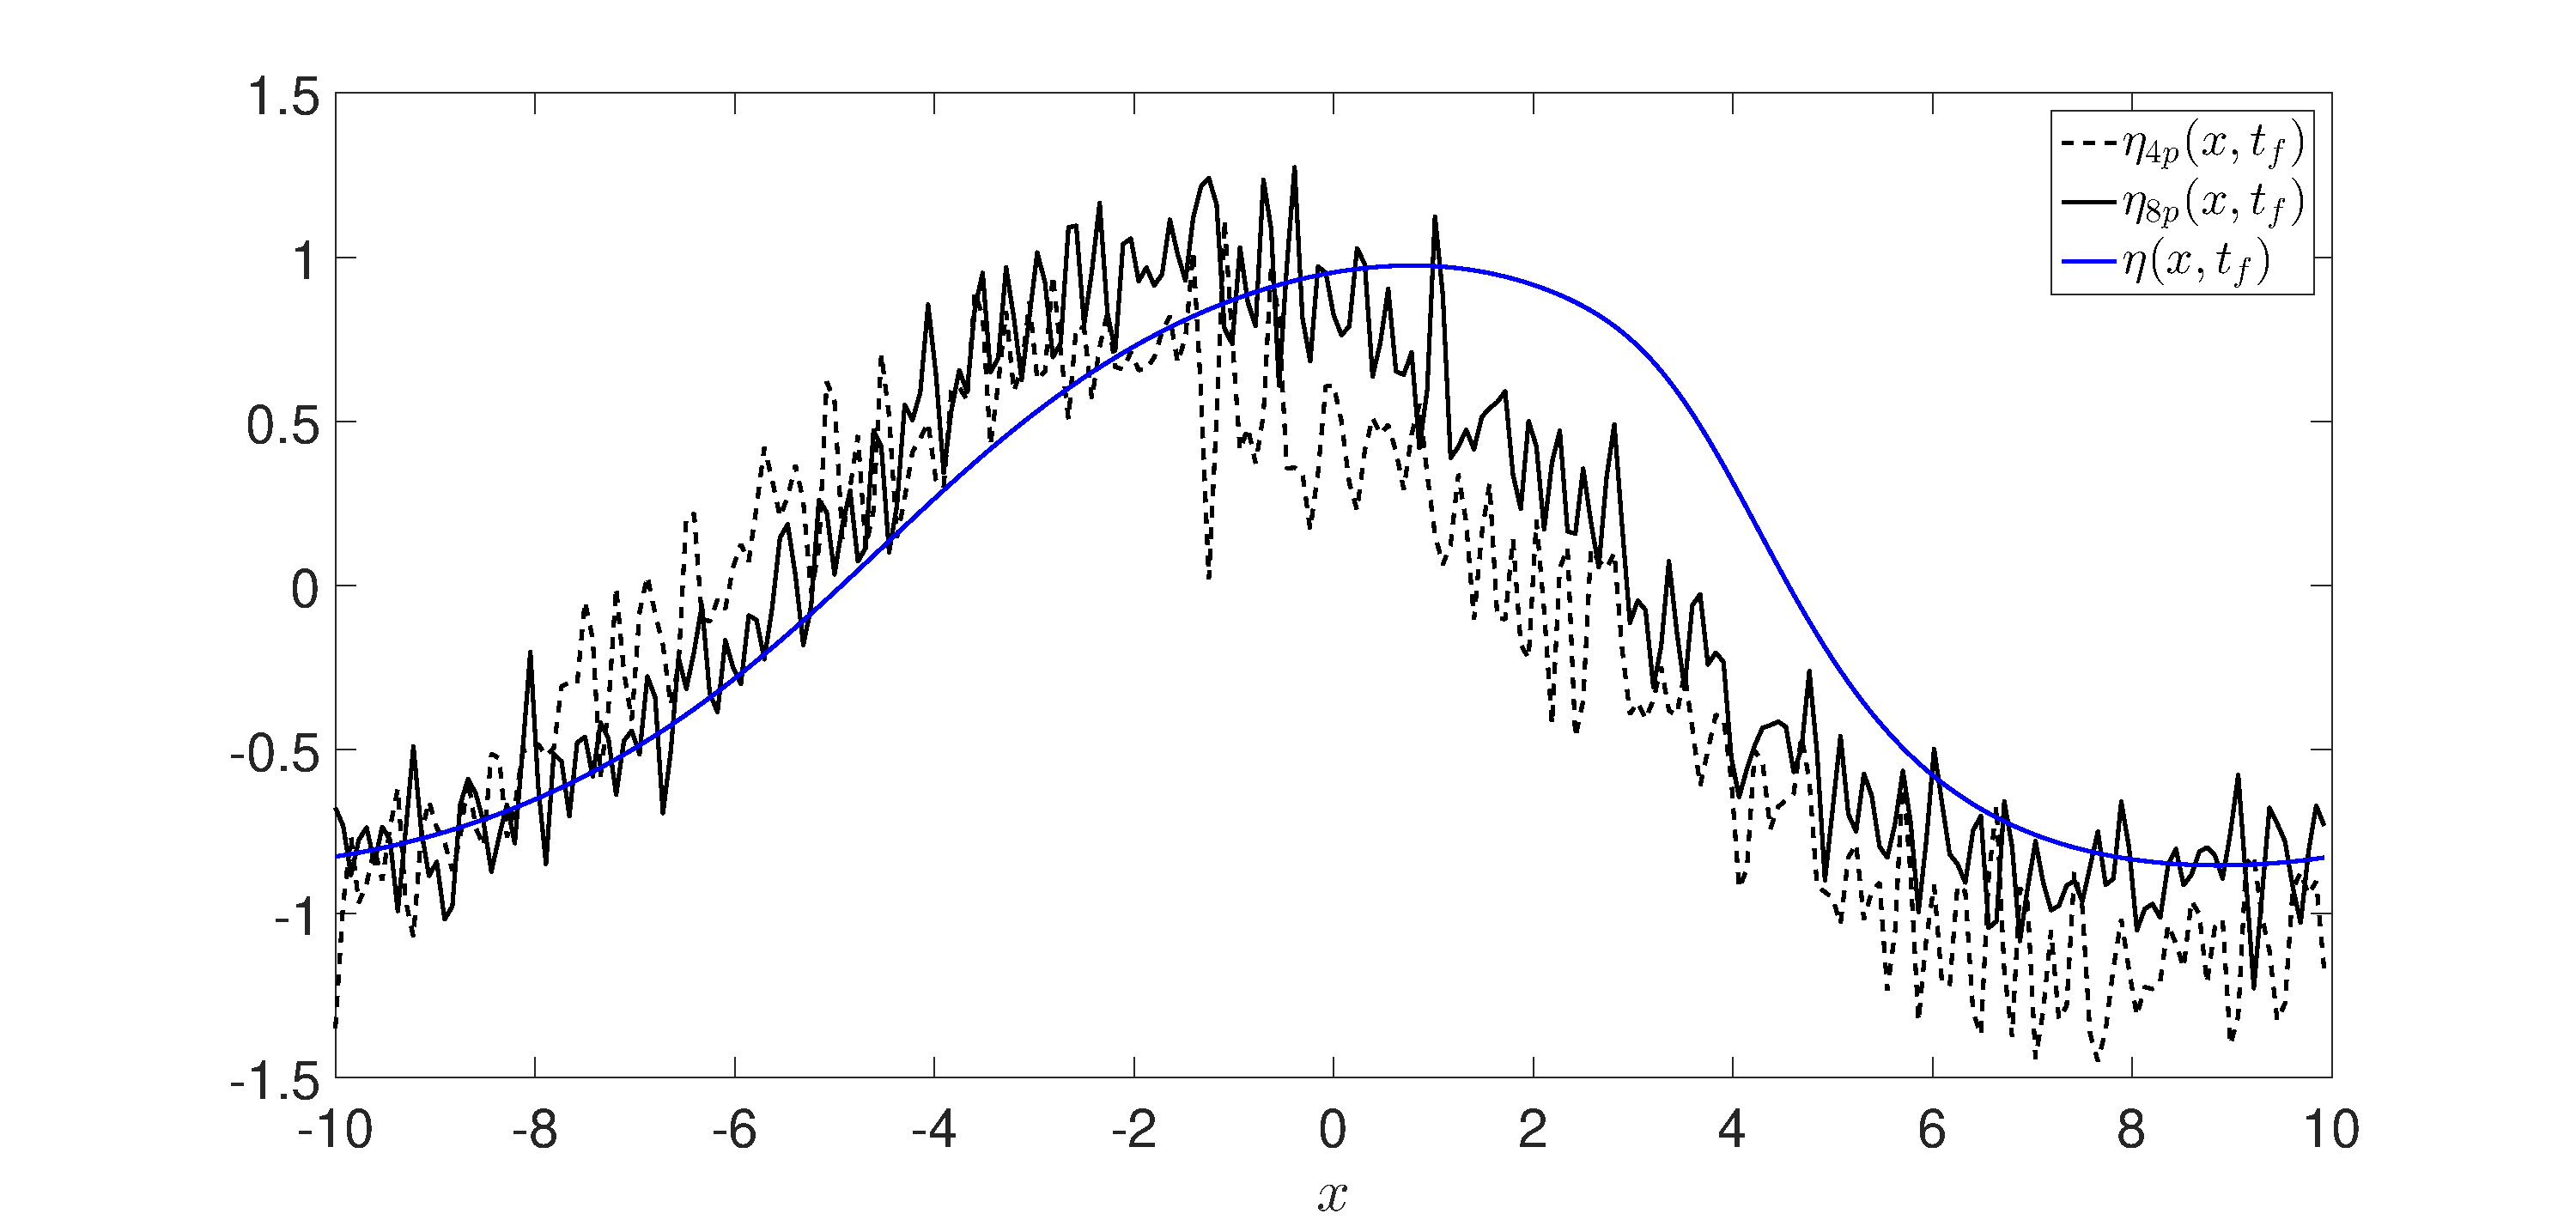
\includegraphics[width=.95\textwidth]{Images/wave_tf_20_sig_pt1_4_vs8pplates_Mval_14} \\
(a)\\
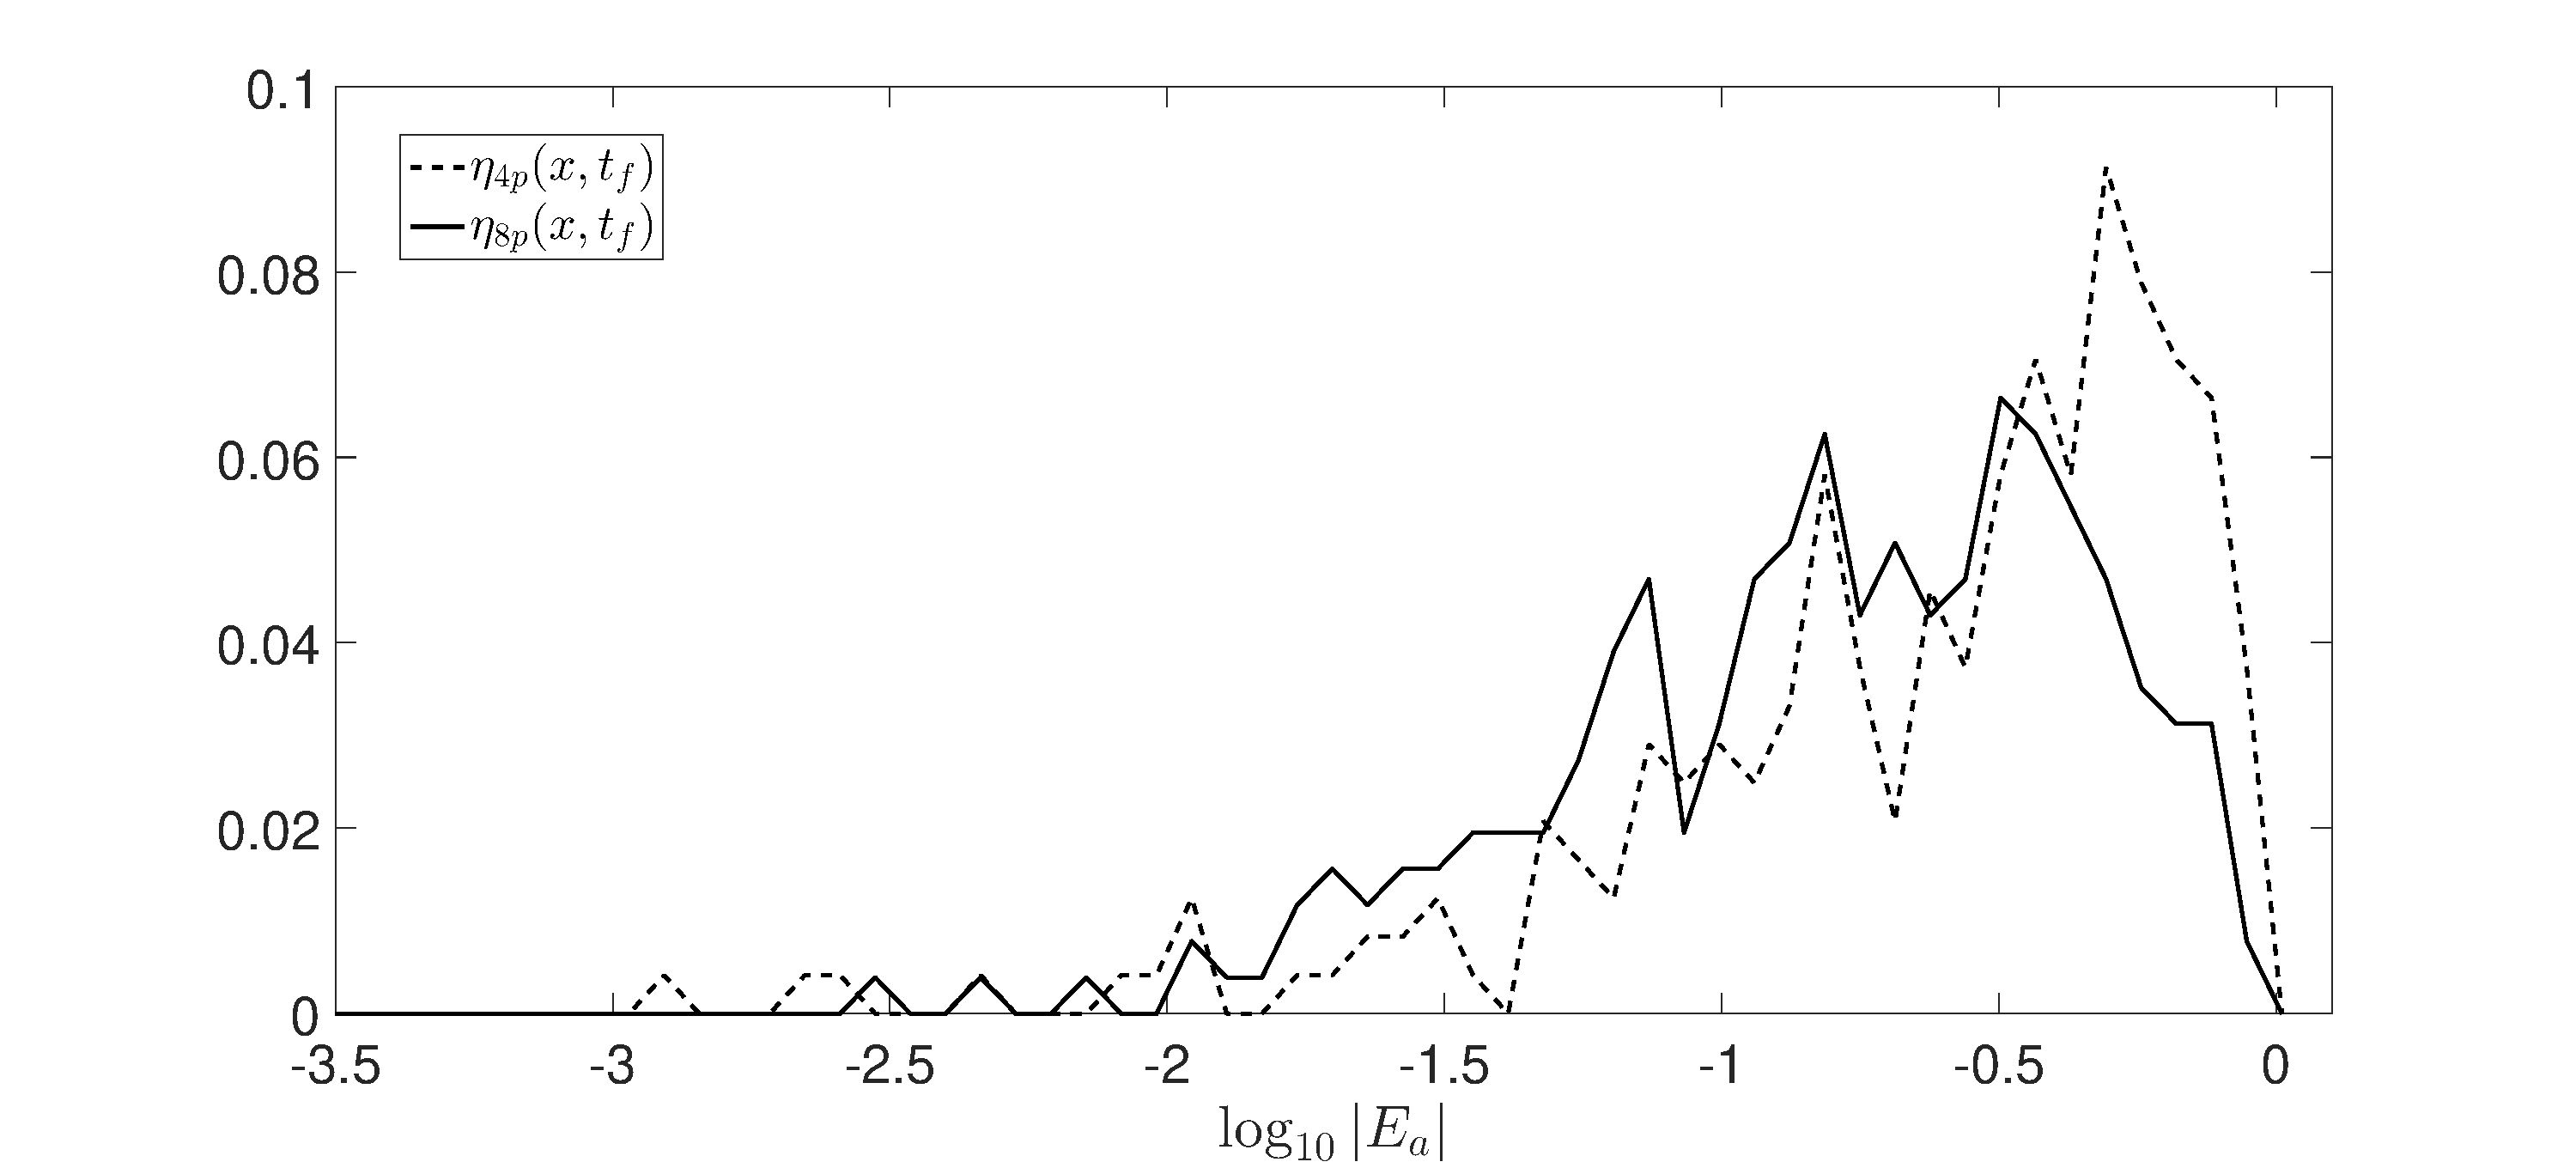
\includegraphics[width=.95\textwidth]{Images/histogram_tf_20_sig_pt1_4_vs8pplates_Mval_14}\\
(b)\\
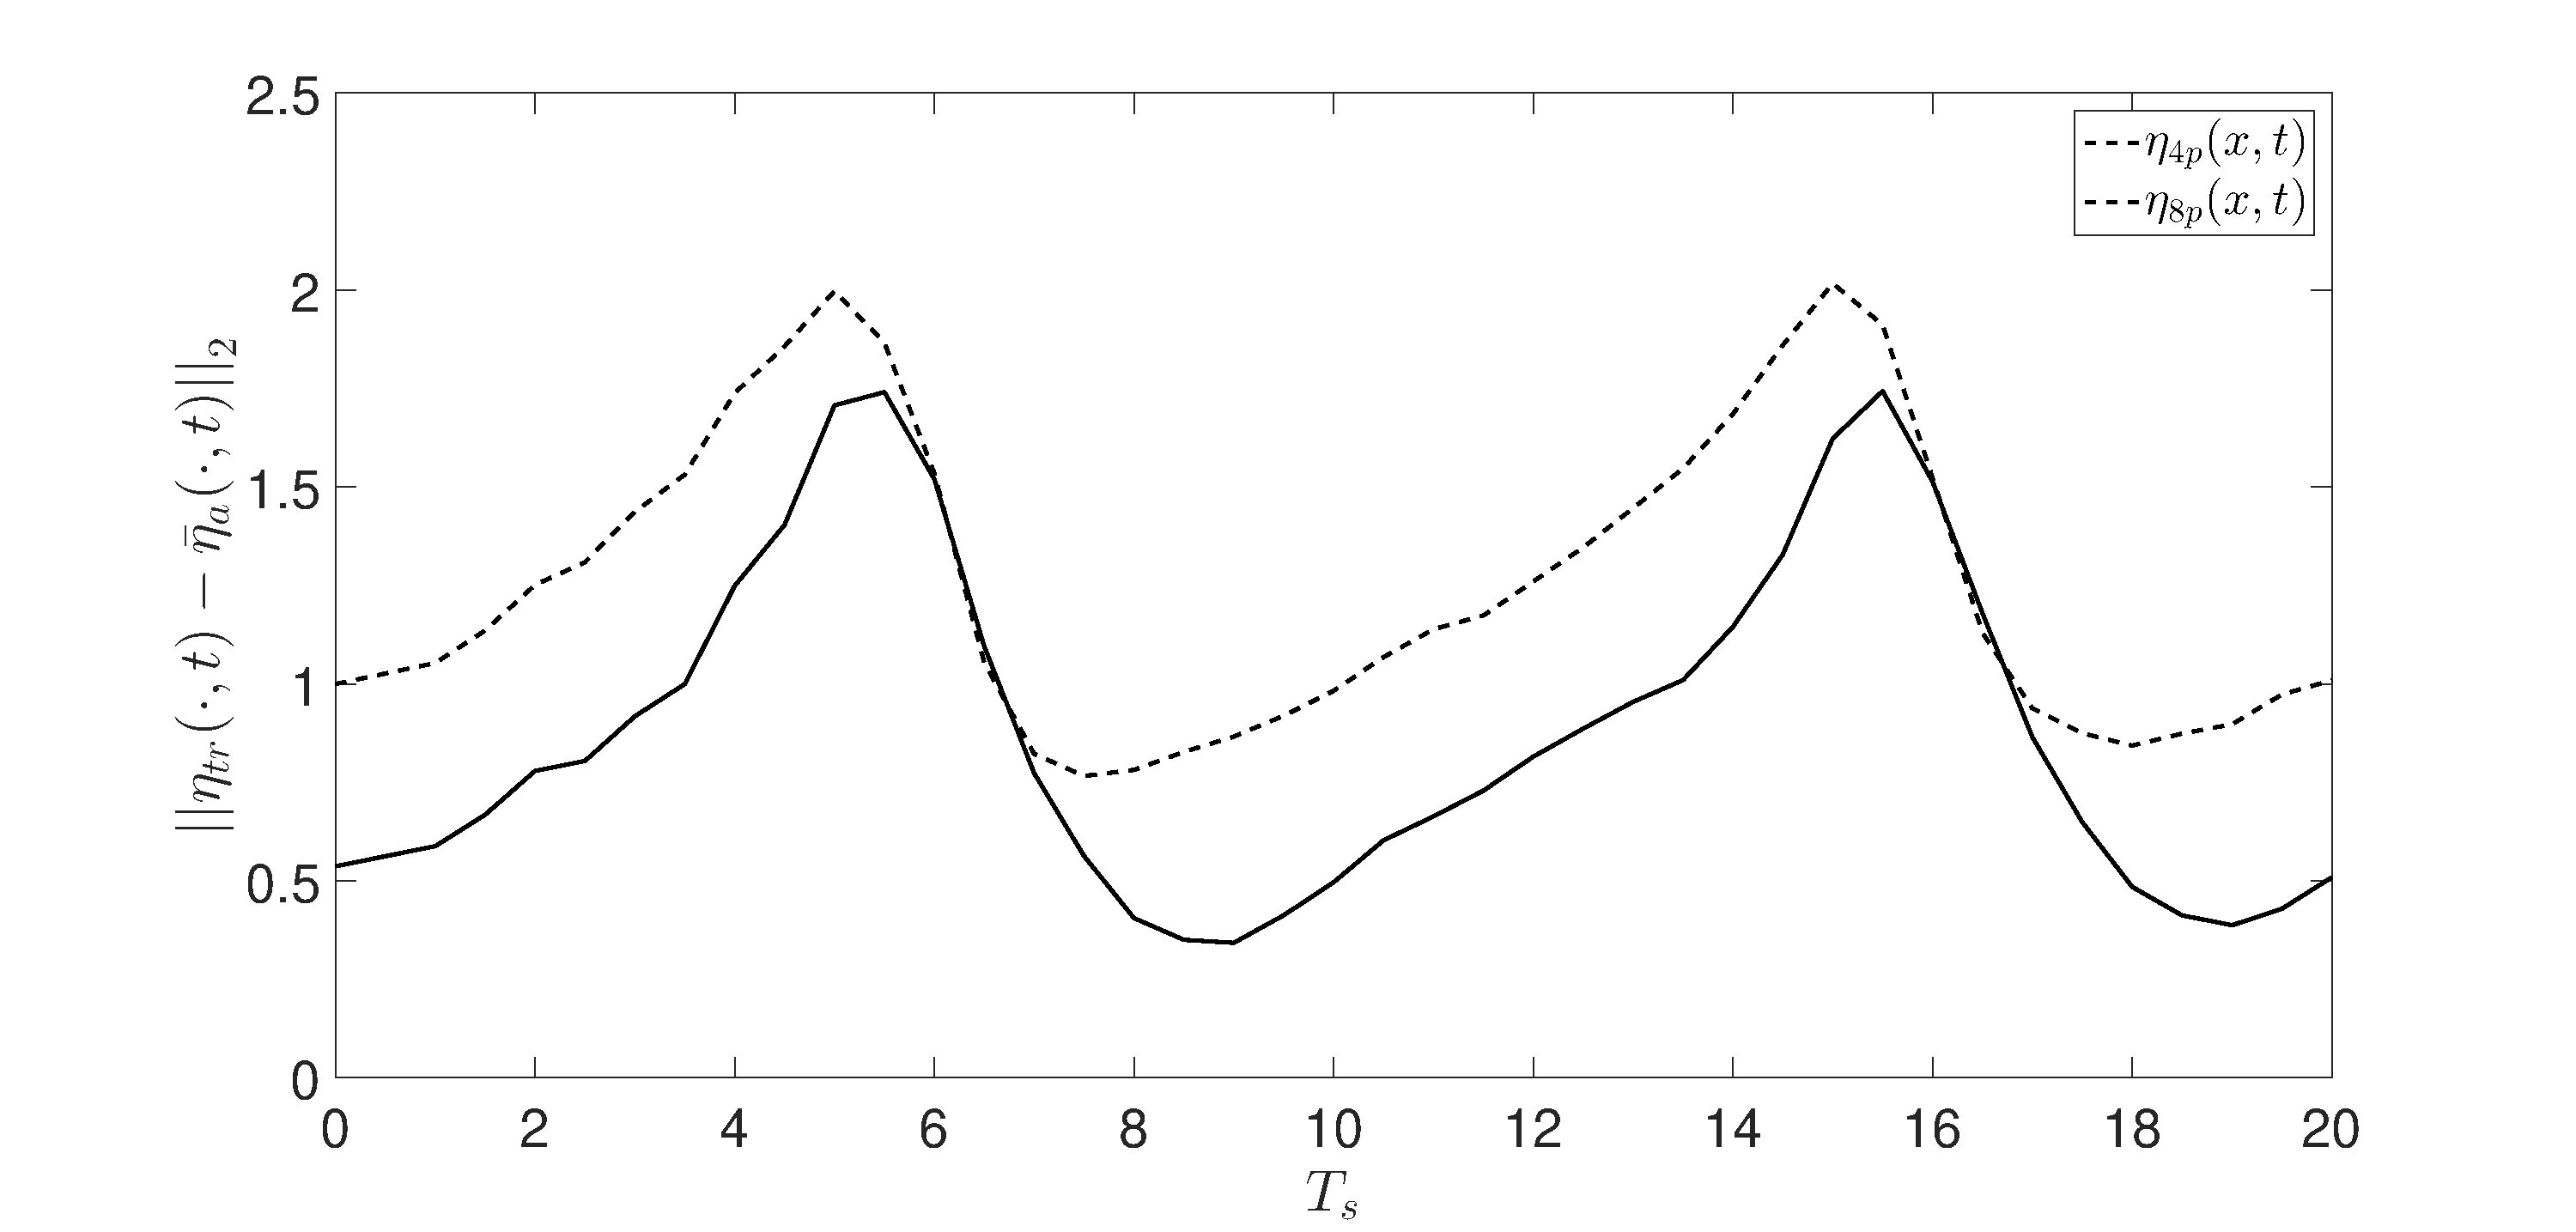
\includegraphics[width=.95\textwidth]{Images/rmserr_tf_20_sig_pt1_4_vs8pplates_Mval_14}\\
(c)
\end{tabular}
\caption{For $M=14$, $dt_{s}=.5$, with four plates (--) compared to eight (-), we have the wave profiles at $t_{f}=20$ (a), a histogram of the log of the pointwise error (b), and the root-square error at every sampling time (c).} 
\label{fig:Mval_14}
\end{figure}

%%%%%%%%%%%%%%%%%%%%%%%%%%%%%%%%%%%%%%%%%%%%%%%%%%%%%%%%%%%%%%%%%%%%%%%%%%%%%%%%%%%


\subsection*{Lagrangian Data Assimilation}
The dynamical system determining surface particle paths is given by the ODEs
\[
\frac{dx}{dt} = \frac{\epsilon\left(q_{x}-\epsilon\mu^{2}\eta_{x}\eta_{t}\right)}{1 + \epsilon^{2}\mu^{2}\eta_{x}^{2}}, ~ \frac{dz}{dt} = \frac{\epsilon\left(\eta_{t}+\epsilon \eta_{x} q_{x}\right)}{1 + \epsilon^{2}\mu^{2}\eta_{x}^{2}}. 
\]
These equations, coupled with the numerical method explained above, allow for the incorporation of surface height measurements following the Lagrangian data assimilation framework advanced in \cite{jones1,jones2}.  

\begin{figure}
	\centering
	\begin{tabular}{c}
		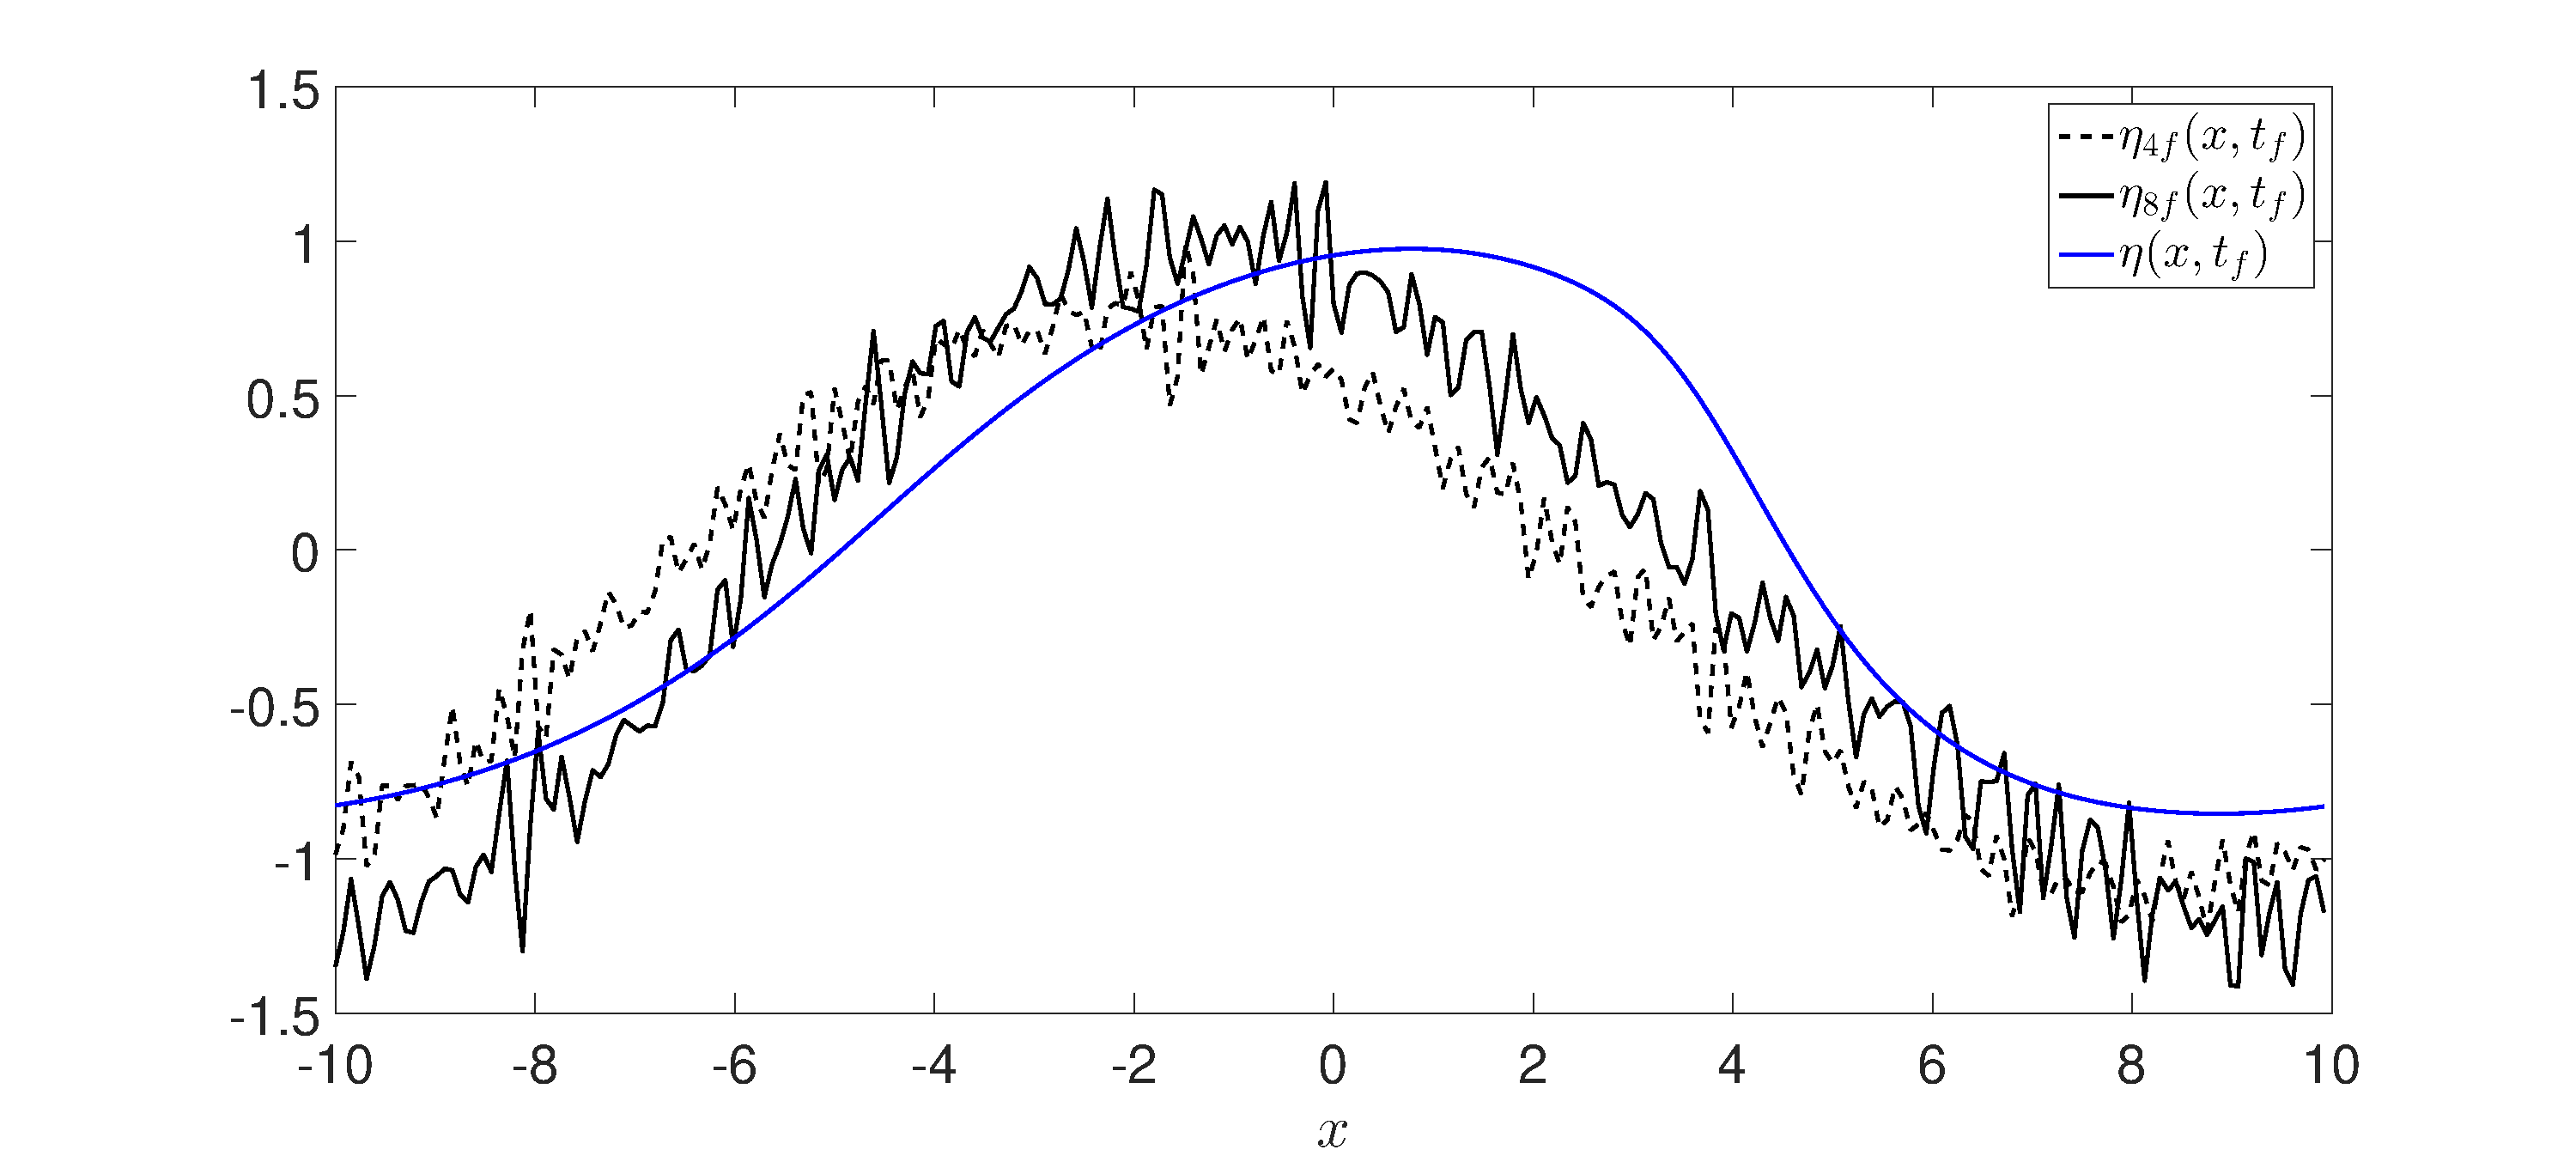
\includegraphics[width=.95\textwidth]{Images/wave_tf_20_sig_pt1_4_vs8floats_Mval_1} \\
		(a)\\
		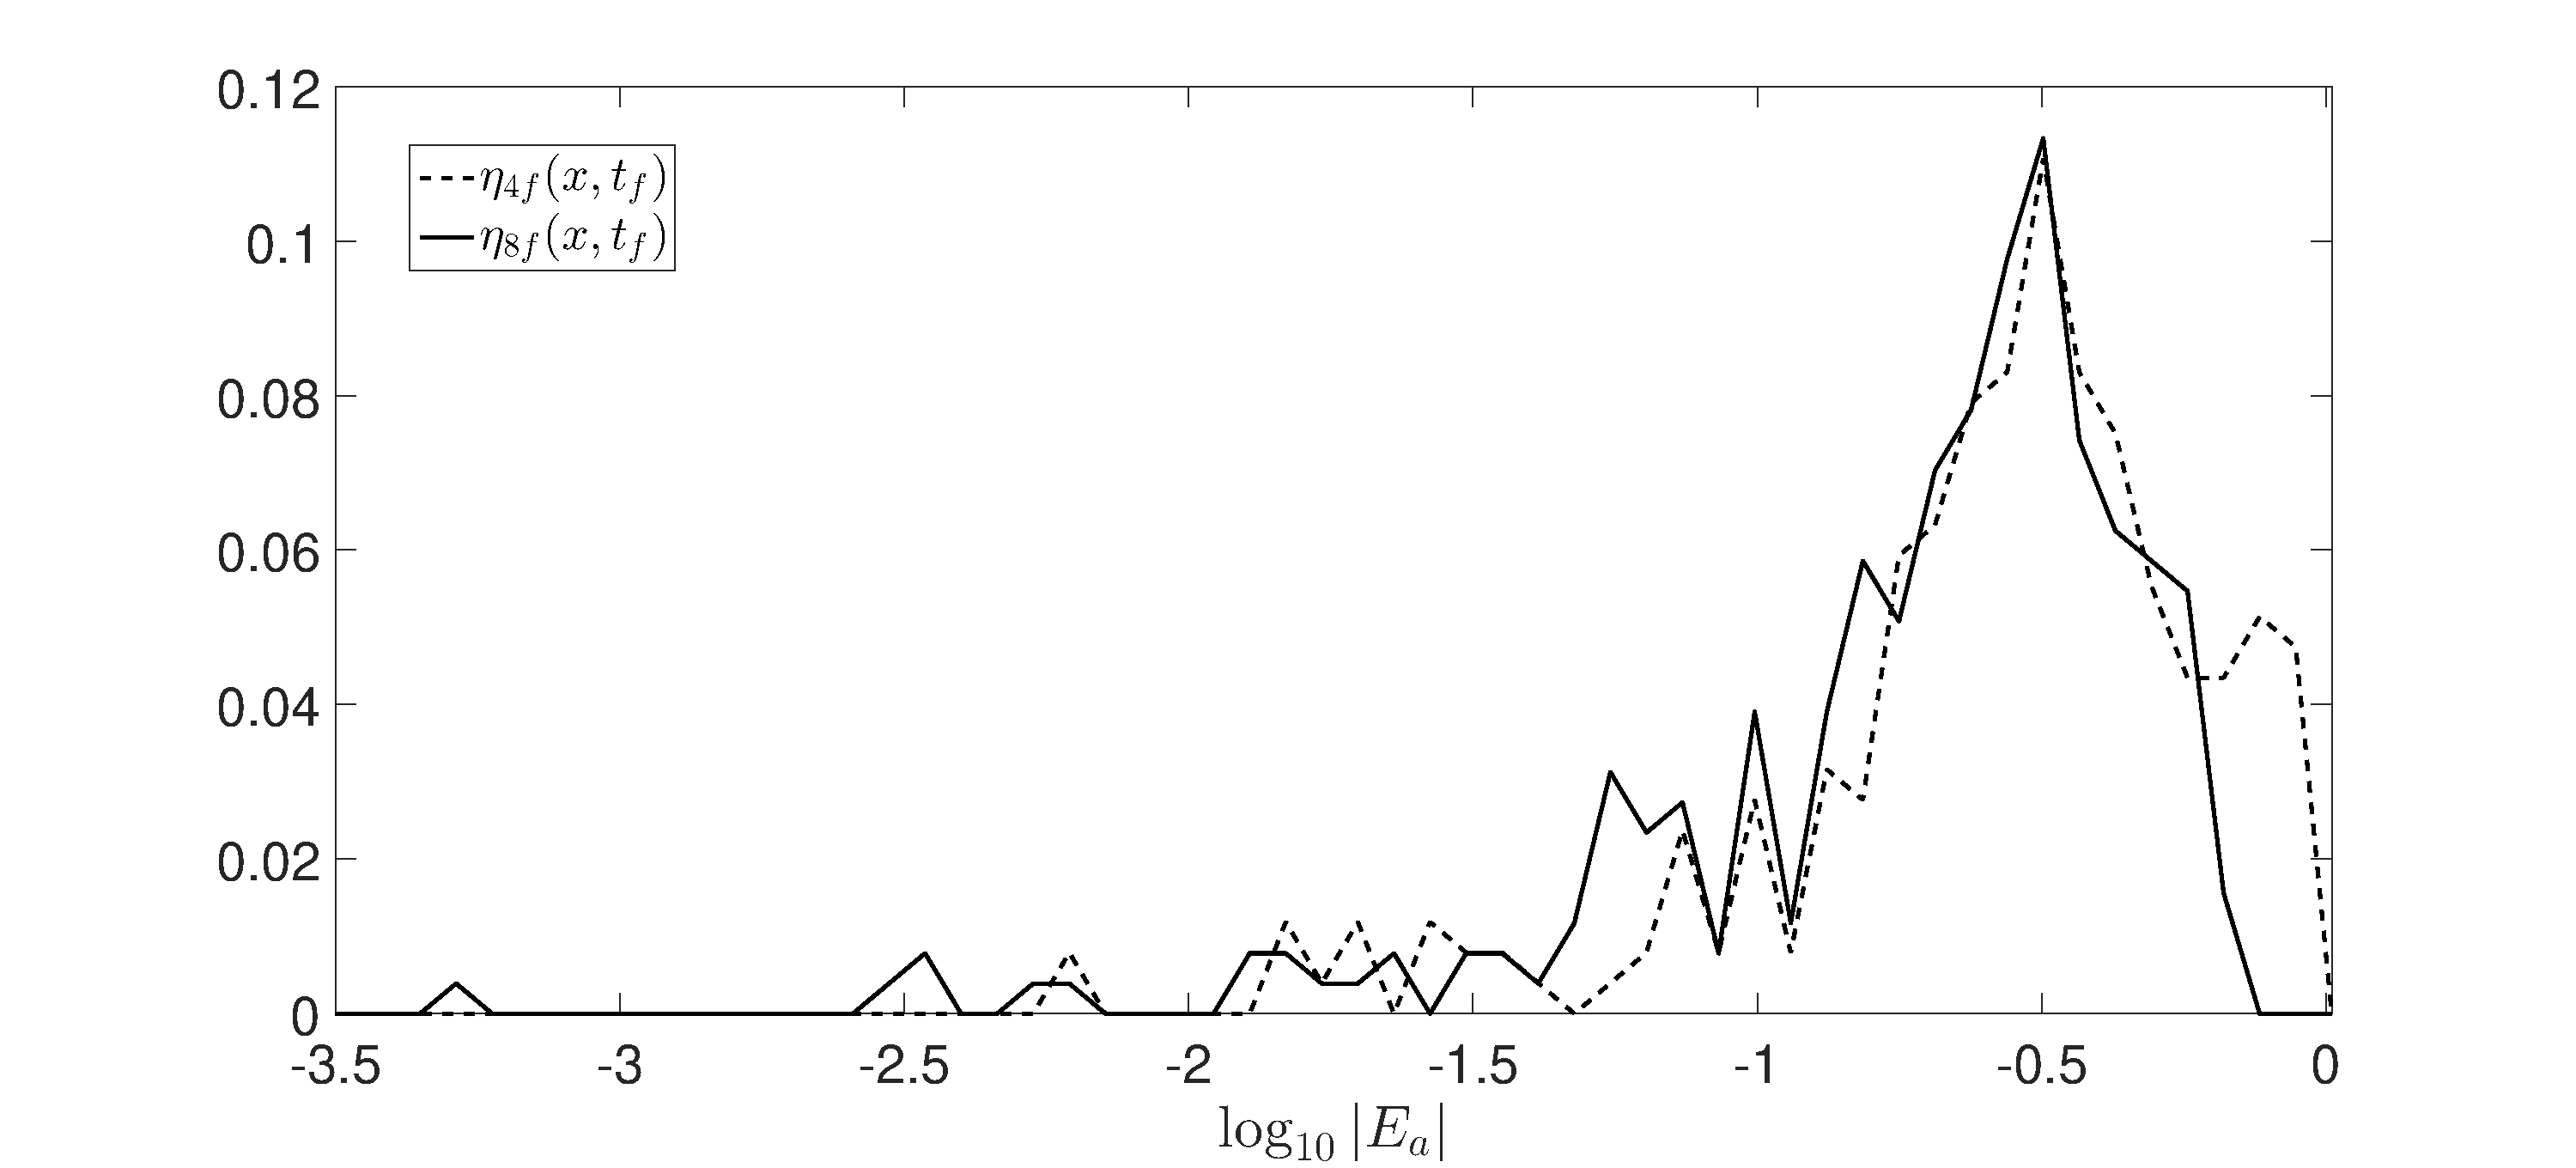
\includegraphics[width=.95\textwidth]{Images/histogram_tf_20_sig_pt1_4_vs_8floats_Mval_1}\\
		(b)\\
		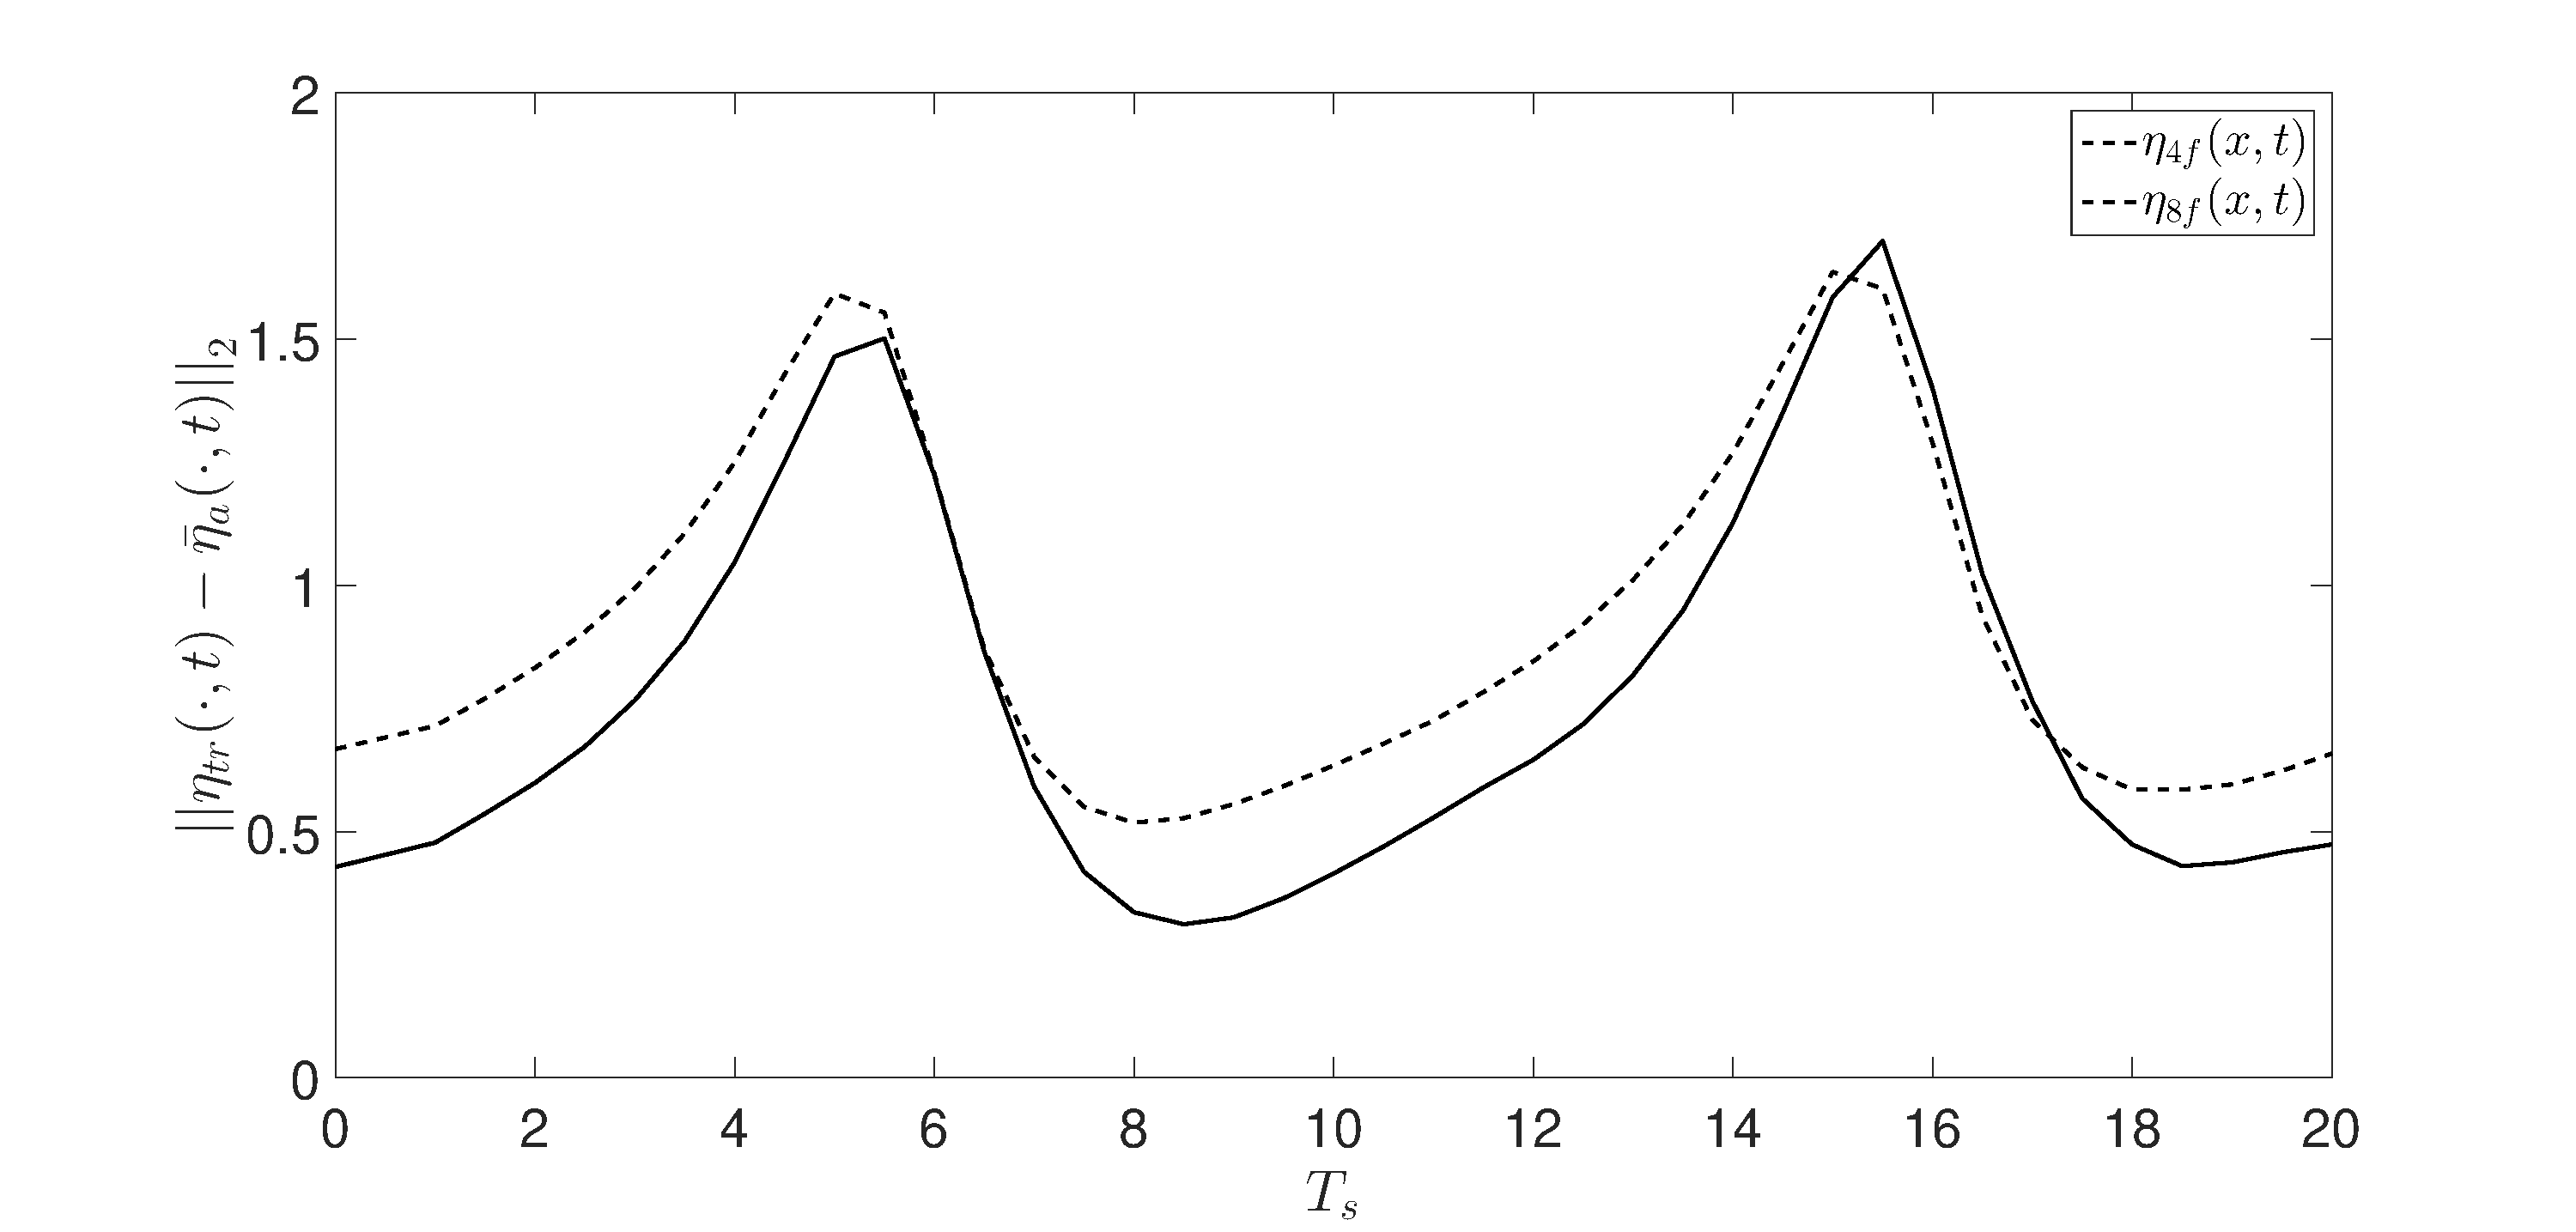
\includegraphics[width=.95\textwidth]{Images/rmserr_tf_20_sig_pt1_4_vs8floats_Mval_1}\\
		(c)
	\end{tabular}
	\caption{For $M=1$, $dt_{s}=.5$, with four floats (--) compared to eight (-), we have the wave profiles at $t_{f}=20$ (a), a histogram of the log of the pointwise error (b), and the root-mean square error at every sampling time (c).} 
	\label{fig:Mval_1}
\end{figure}

\begin{figure}
	\centering
	\begin{tabular}{c}
		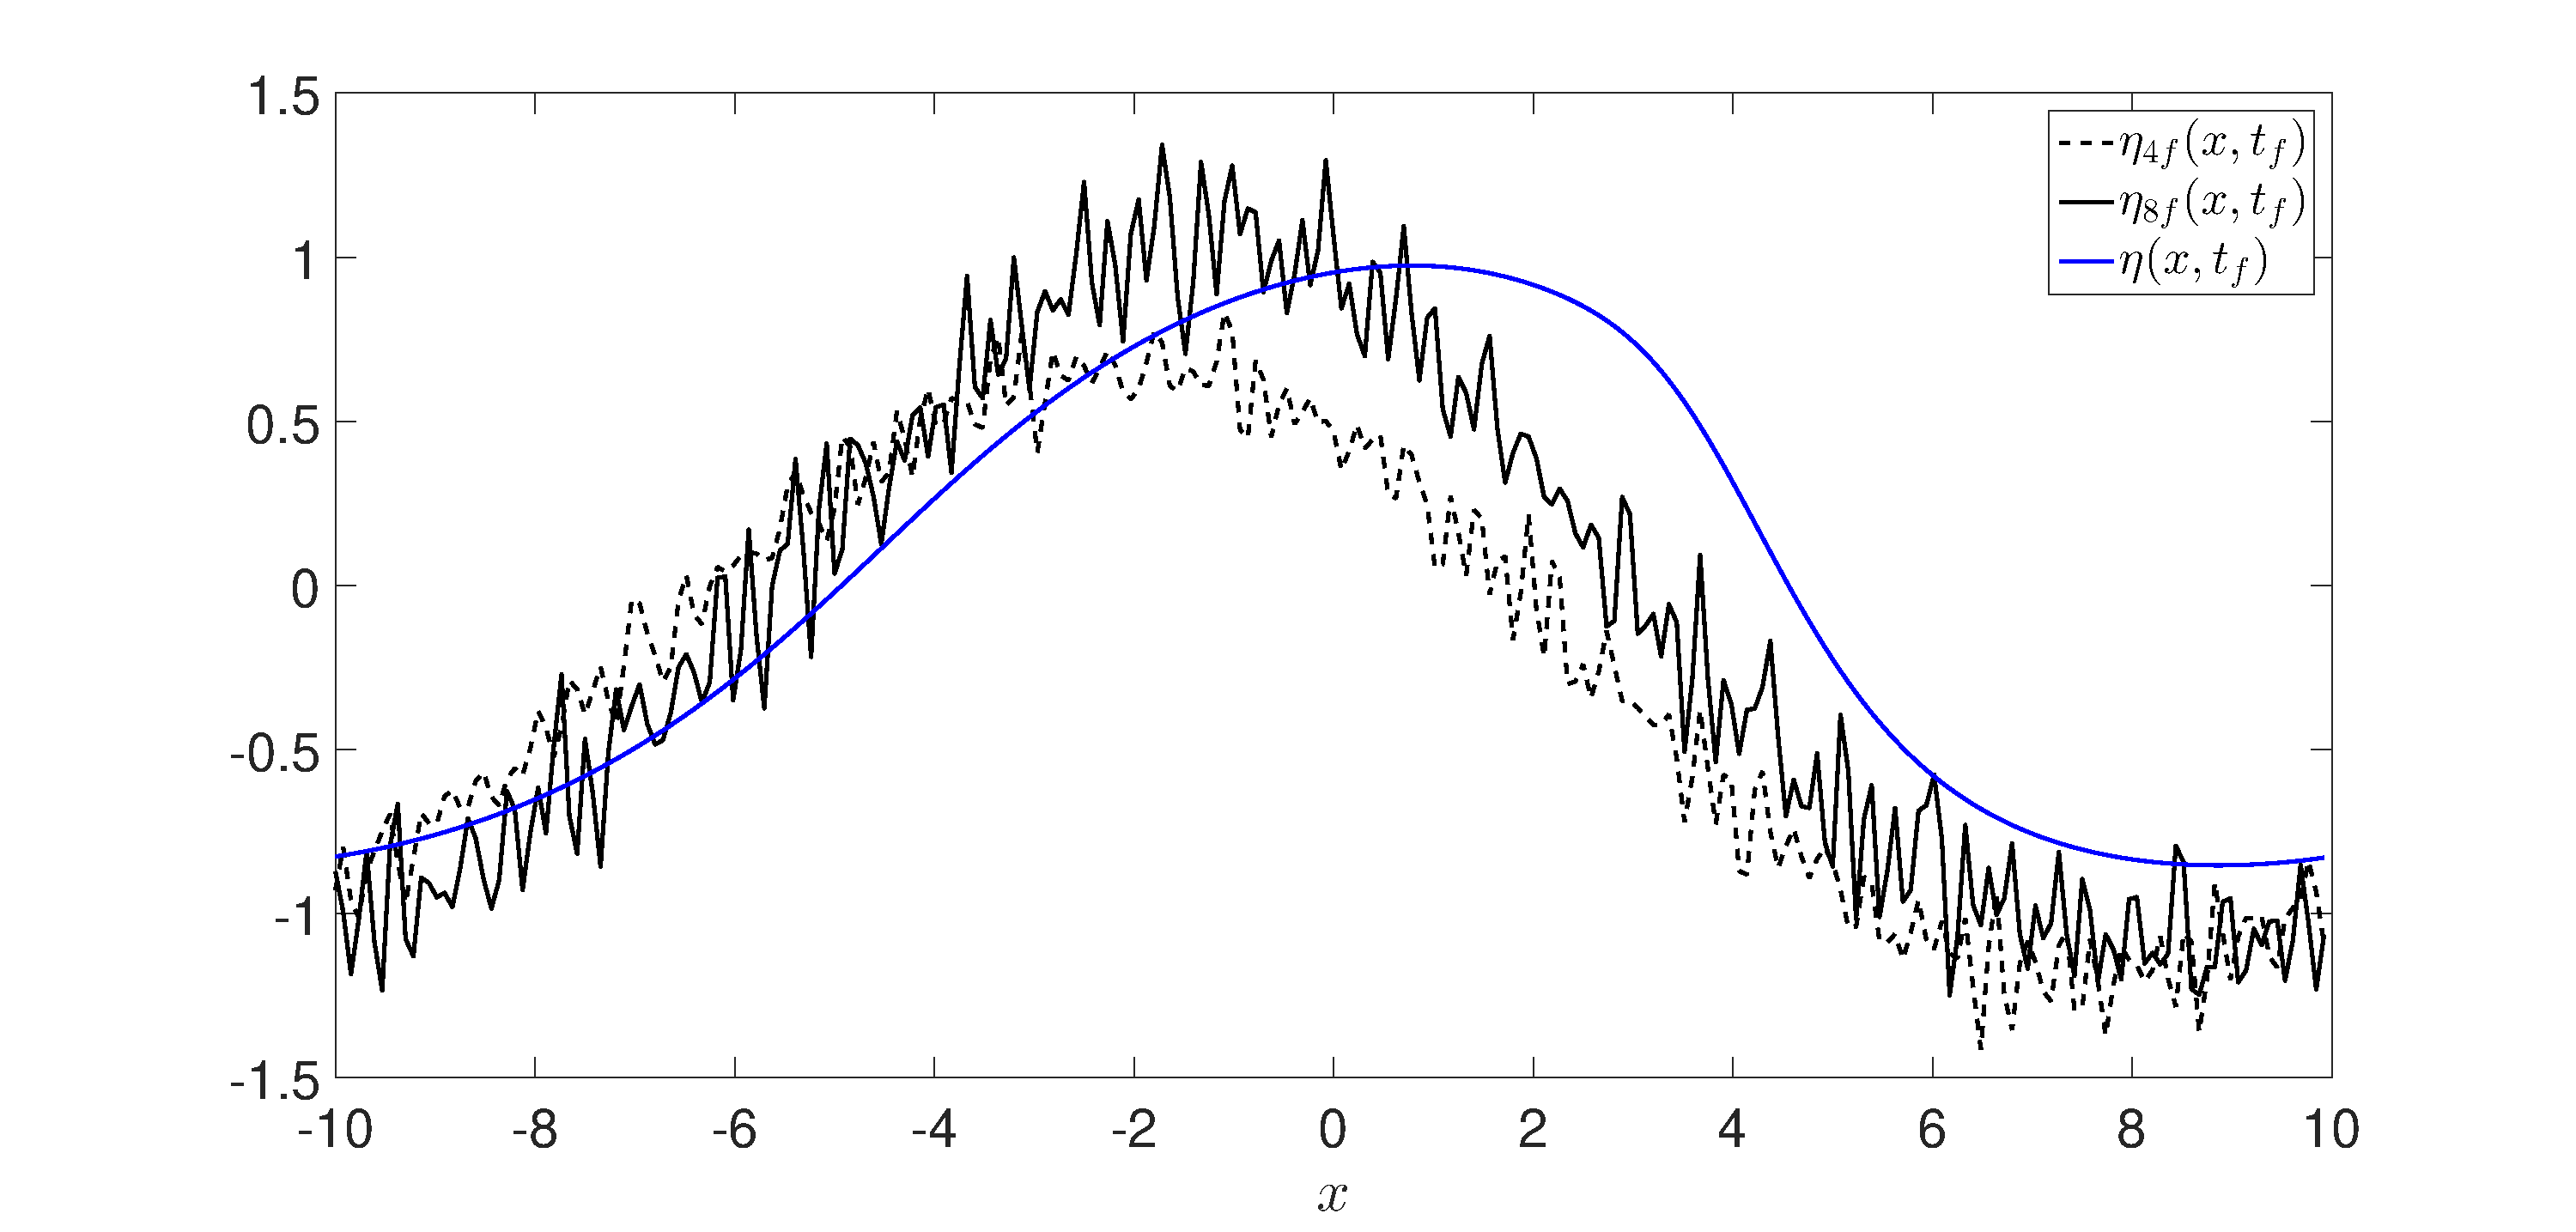
\includegraphics[width=.95\textwidth]{Images/wave_tf_20_sig_pt1_4_vs8floats_Mval_14} \\
		(a)\\
		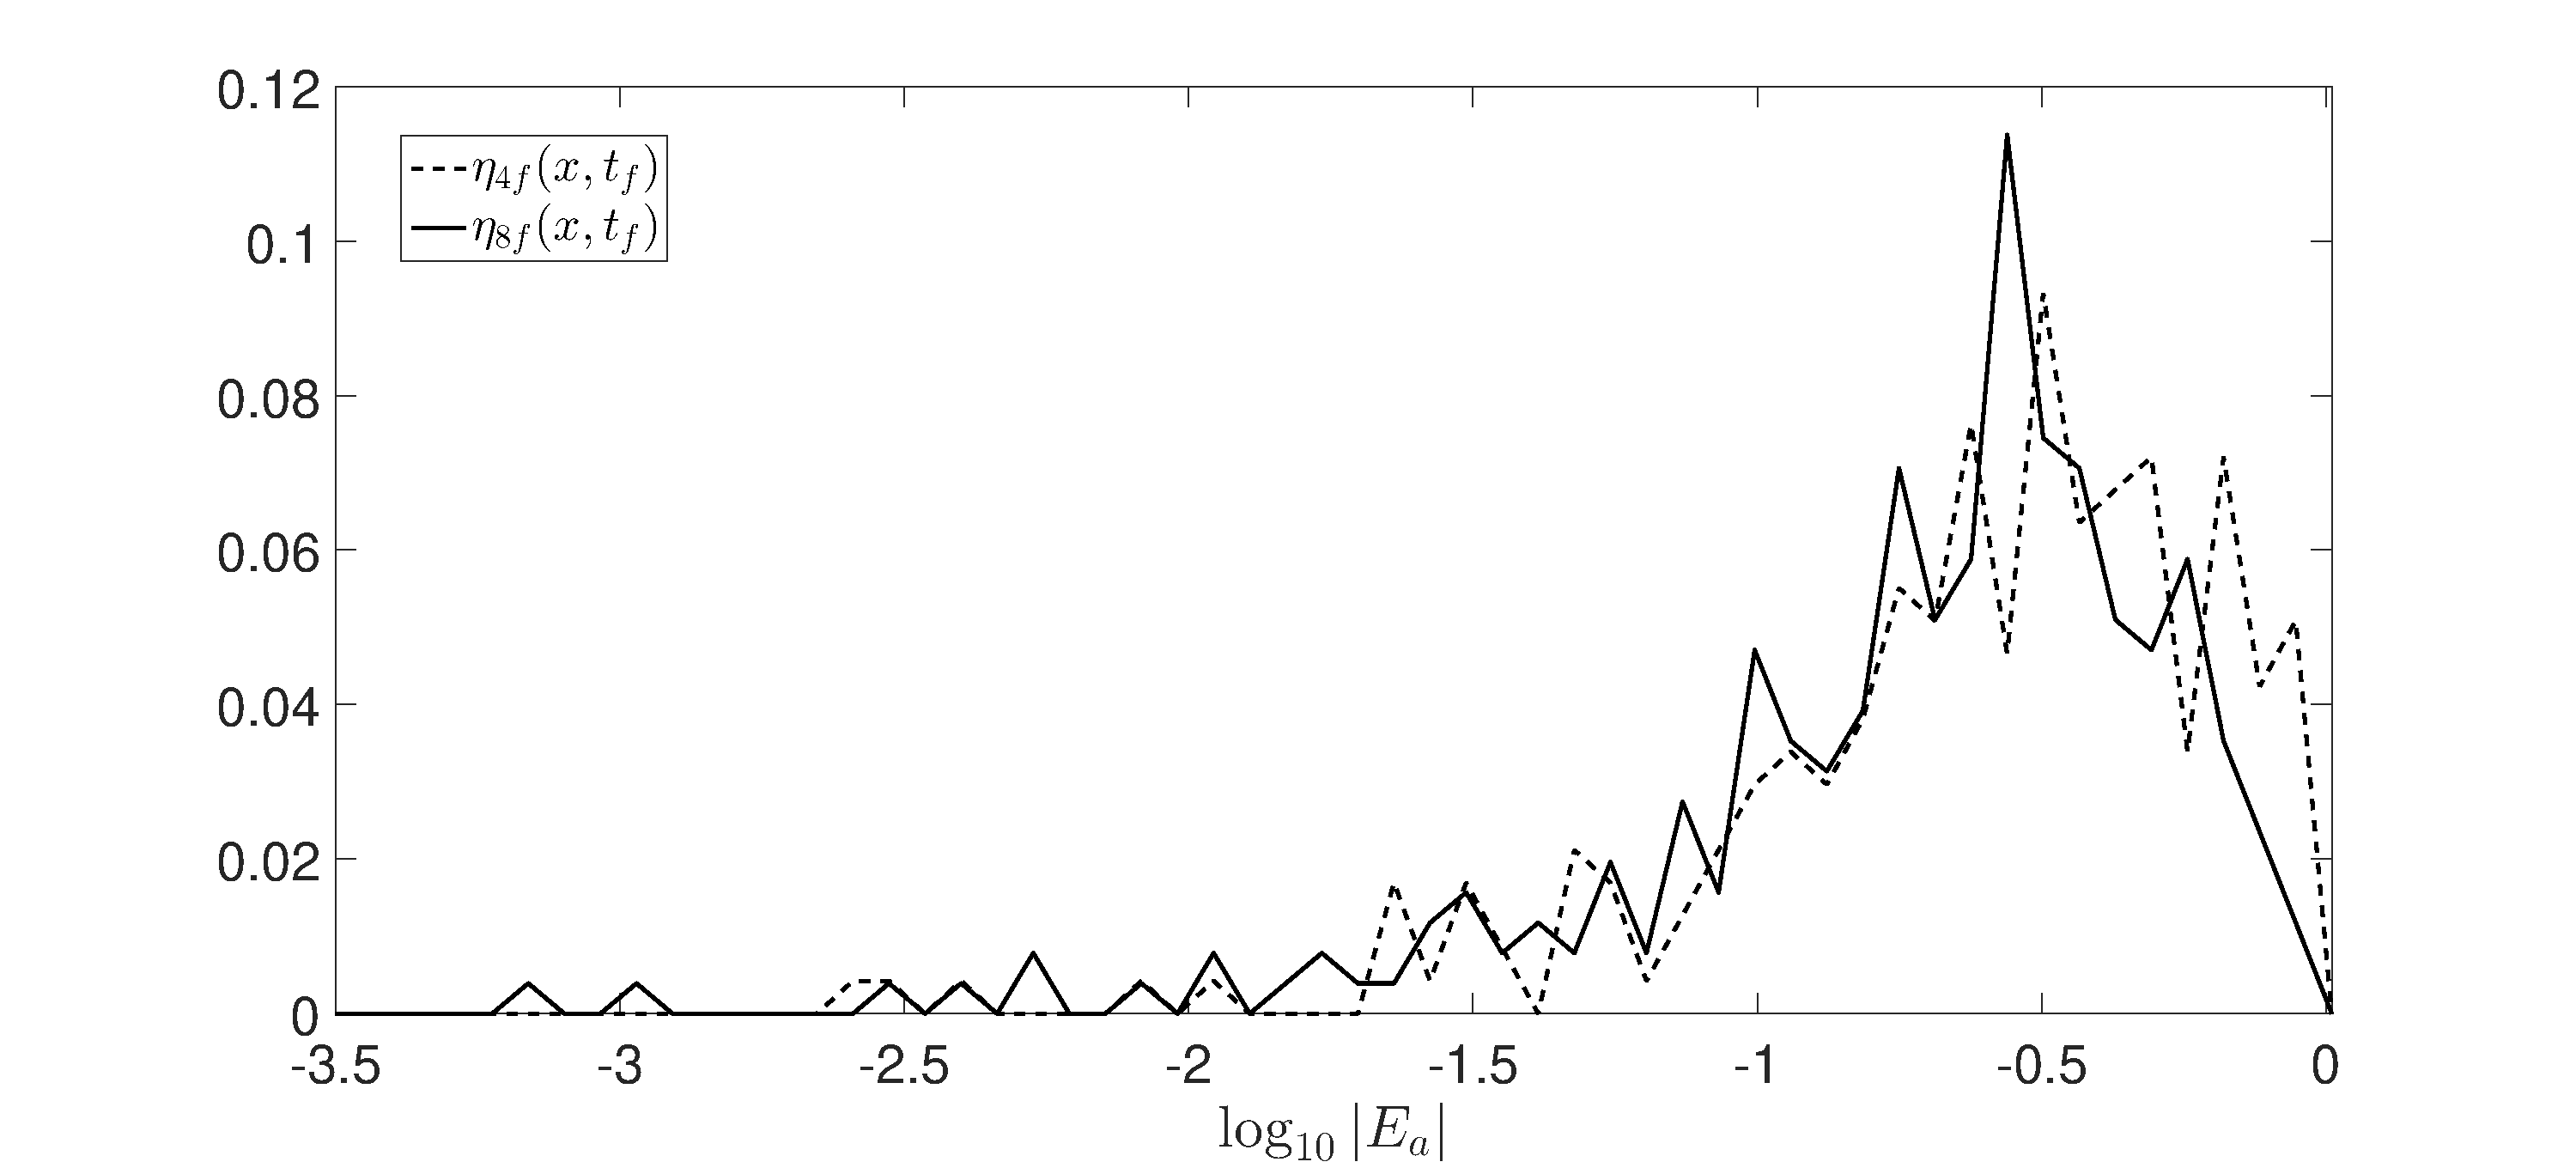
\includegraphics[width=.95\textwidth]{Images/histogram_tf_20_sig_pt1_4_vs_8floats_Mval_14}\\
		(b)\\
		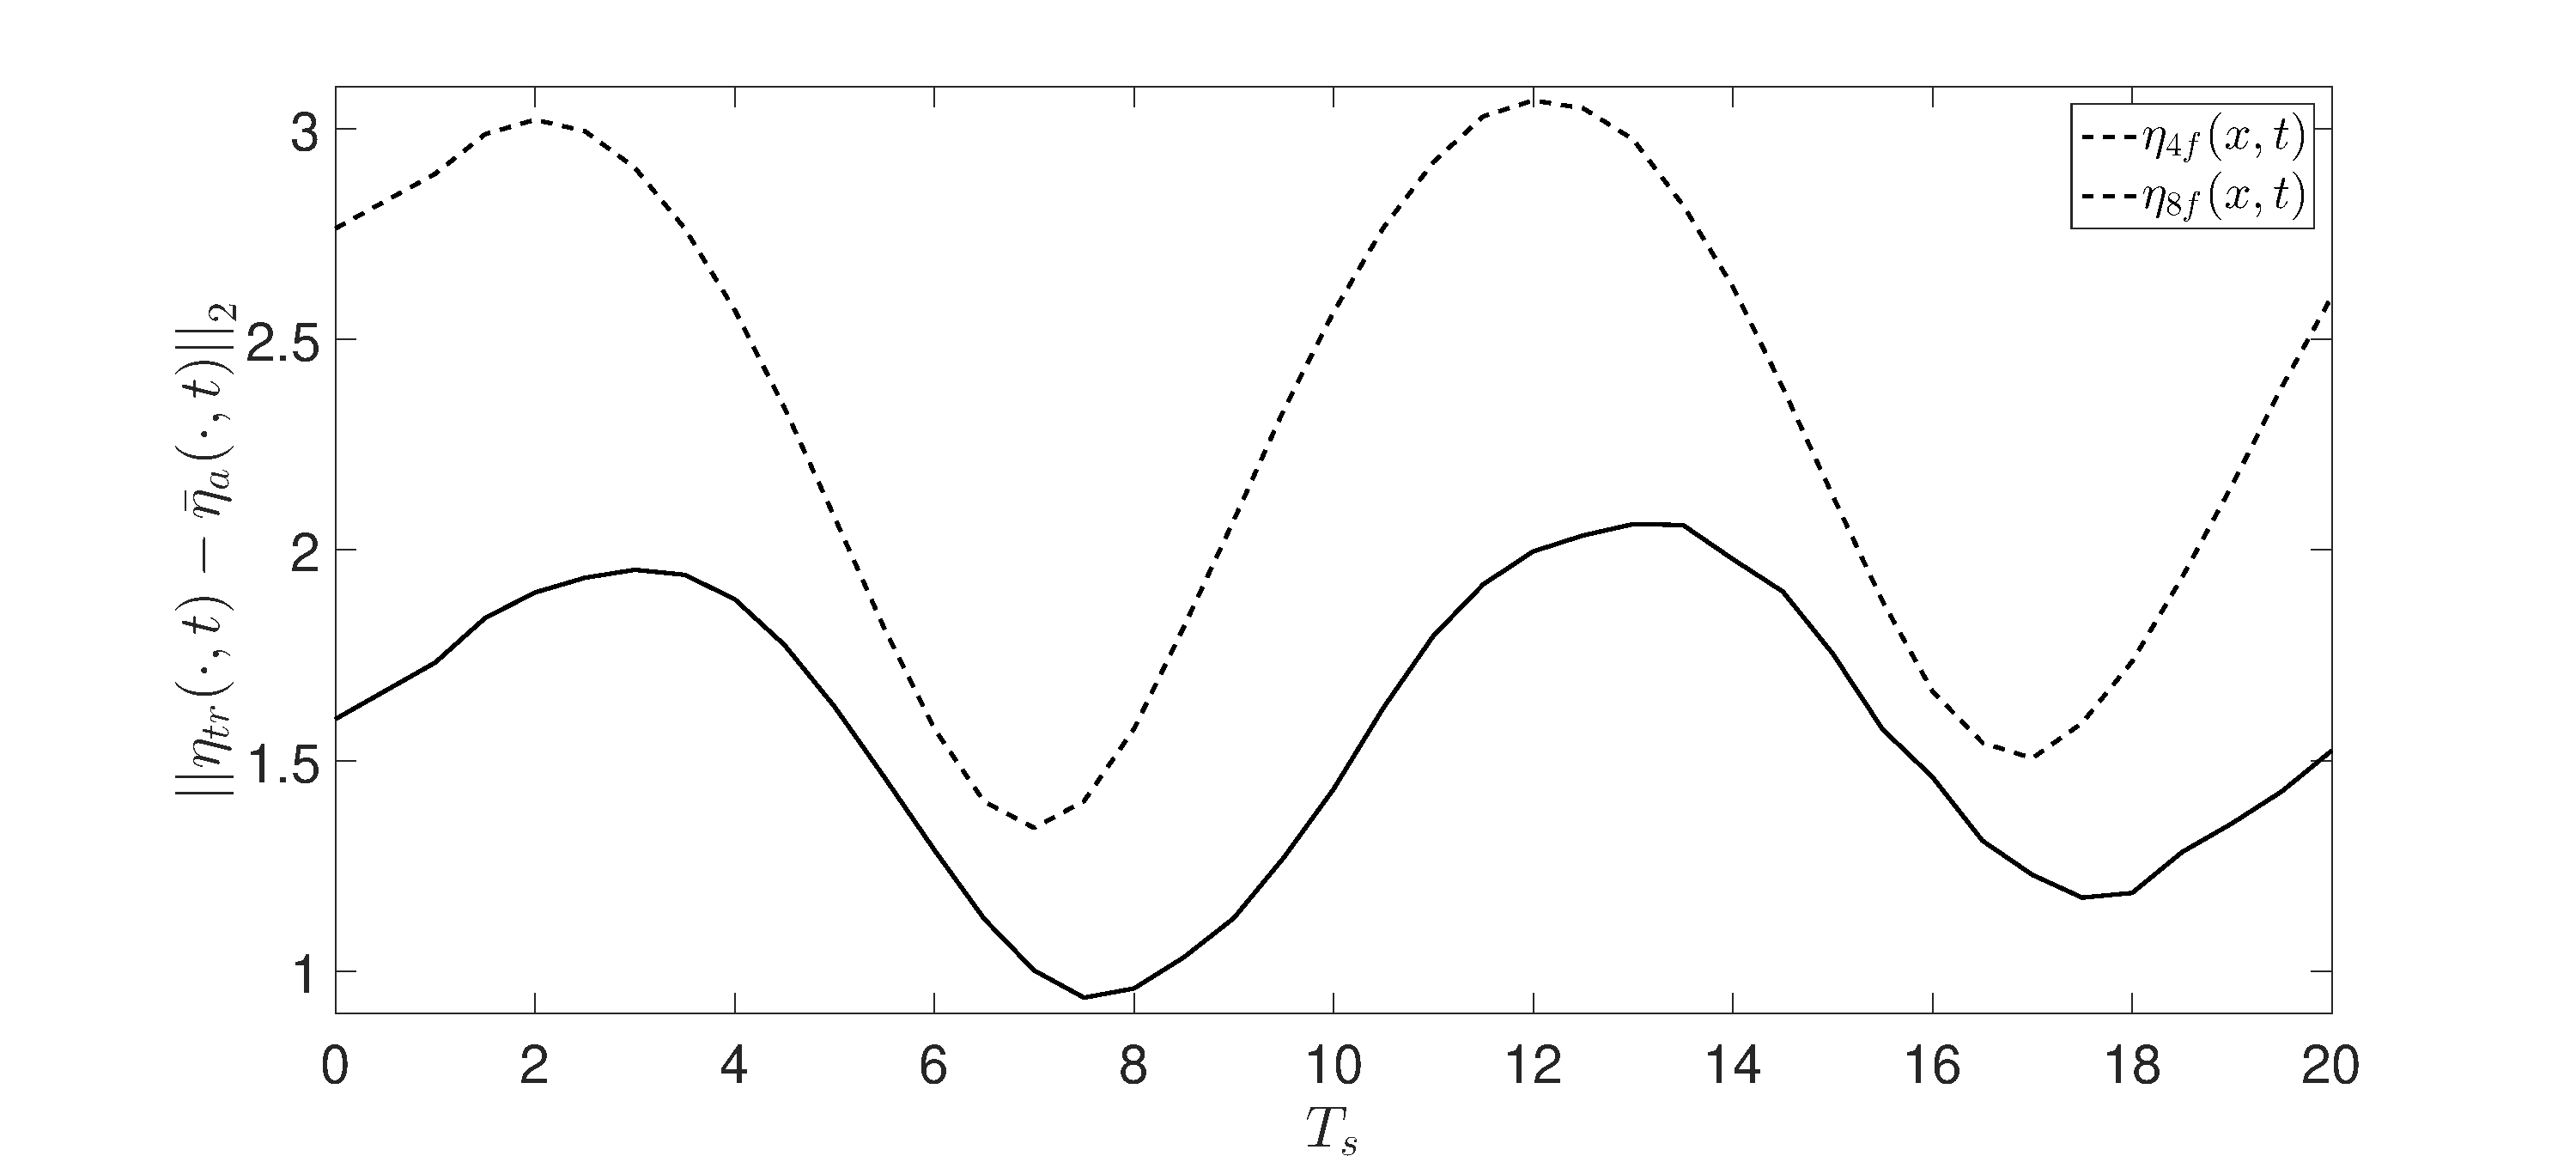
\includegraphics[width=.95\textwidth]{Images/rmserr_tf_20_sig_pt1_4_vs8floats_Mval_14}\\
		(c)
	\end{tabular}
	\caption{For $M=1$, $dt_{s}=.5$, with four floats (--) compared to eight (-), we have the wave profiles at $t_{f}=20$ (a), a histogram of the log of the pointwise error (b), and the root-square error at every sampling time (c).} 
	\label{fig:Mval_1}
\end{figure}
